%% History:
% Pavel Tvrdik (26.12.2004)
%  + initial version for PhD Report
%
% Daniel Sykora (27.01.2005)
%
% Michal Valenta (3.12.2008)
% rada zmen ve formatovani (diky M. Duškovi, J. Holubovi a J. Žďárkovi)
% sjednoceni zdrojoveho kodu pro anglickou, ceskou, bakalarskou a diplomovou praci

% One-page layout: (proof-)reading on display
%%%% \documentclass[11pt,oneside,a4paper]{book}
% Two-page layout: final printing
\documentclass[11pt,twoside,a4paper]{book}   

\usepackage{wrapfig, floatrow, amsmath, url, graphicx}

\usepackage[czech, english]{babel}
\usepackage[T1]{fontenc} % pouzije EC fonty 
% pripadne pisete-li cesky, pak lze zkusit take:
% \usepackage[OT1]{fontenc} 
\usepackage[utf8]{inputenc}
%=-=-=-=-=-=-=-=-=-=-=-=--=%
% In case of problems with PDF fonts, one may try to uncomment this line:
%\usepackage{lmodern}
%=-=-=-=-=-=-=-=-=-=-=-=--=%
%=-=-=-=-=-=-=-=-=-=-=-=--=%
% Depending on your particular TeX distribution and version of conversion tools 
% (dvips/dvipdf/ps2pdf), some (advanced | desperate) users may prefer to use 
% different settings.
% Please uncomment the following style and use your CSLaTeX (cslatex/pdfcslatex) 
% to process your work. Note however, this file is in UTF-8 and a conversion to 
% your native encoding may be required. Some settings below depend on babel 
% macros and should also be modified. See \selectlanguage \iflanguage.
%\usepackage{czech}  %%%%%\usepackage[T1]{czech} %%%%[IL2] [T1] [OT1]
%=-=-=-=-=-=-=-=-=-=-=-=--=%

%%%%%%%%%%%%%%%%%%%%%%%%%%%%%%%%%%%%%%%
% Styles required in your work follow %
%%%%%%%%%%%%%%%%%%%%%%%%%%%%%%%%%%%%%%%
\usepackage{graphicx}
\usepackage{indentfirst} %1. odstavec jako v cestine.
\usepackage{listings}
\renewcommand{\lstlistingname}{Ukázka}
\lstset{
  frame=top,frame=bottom,
  basicstyle=\small\normalfont\sffamily,    % the size of the fonts that are used for the code
  stepnumber=1,                           % the step between two line-numbers. If it is 1 each line will be numbered
  numbersep=10pt,                         % how far the line-numbers are from the code
  tabsize=2,                              % tab size in blank spaces
  extendedchars=true,                     %
  breaklines=true,                        % sets automatic line breaking
  captionpos=b,                           % sets the caption-position to top
  mathescape=true,
  stringstyle=\color{white}\ttfamily, % Farbe der String
  showspaces=false,           % Leerzeichen anzeigen ?
  showtabs=false,             % Tabs anzeigen ?
  xleftmargin=17pt,
  xrightmargin=17pt,
  framexleftmargin=17pt,
  framexrightmargin=17pt,
  framexbottommargin=5pt,
  framextopmargin=5pt,
  showstringspaces=false      % Leerzeichen in Strings anzeigen ?
 }
 
\lstdefinelanguage{GLSL}
{
sensitive=true,
morekeywords=[1]{
attribute, const, uniform, varying,
layout, centroid, flat, smooth,
noperspective, break, continue, do,
for, while, switch, case, default, if,
else, in, out, inout, float, int, void,
bool, true, false, invariant, discard,
return, mat2, mat3, mat4, mat2x2, mat2x3,
mat2x4, mat3x2, mat3x3, mat3x4, mat4x2,
mat4x3, mat4x4, vec2, vec3, vec4, ivec2,
ivec3, ivec4, bvec2, bvec3, bvec4, uint,
uvec2, uvec3, uvec4, lowp, mediump, highp,
precision, sampler1D, sampler2D, sampler3D,
samplerCube, sampler1DShadow,
sampler2DShadow, samplerCubeShadow,
sampler1DArray, sampler2DArray,
sampler1DArrayShadow, sampler2DArrayShadow,
isampler1D, isampler2D, isampler3D,
isamplerCube, isampler1DArray,
isampler2DArray, usampler1D, usampler2D,
usampler3D, usamplerCube, usampler1DArray,
usampler2DArray, sampler2DRect,
sampler2DRectShadow, isampler2DRect,
usampler2DRect, samplerBuffer,
isamplerBuffer, usamplerBuffer, sampler2DMS,
isampler2DMS, usampler2DMS,
sampler2DMSArray, isampler2DMSArray,
usampler2DMSArray, struct},
morekeywords=[2]{
radians,degrees,sin,cos,tan,asin,acos,atan,
atan,sinh,cosh,tanh,asinh,acosh,atanh,pow,
exp,log,exp2,log2,sqrt,inversesqrt,abs,sign,
floor,trunc,round,roundEven,ceil,fract,mod,modf,
min,max,clamp,mix,step,smoothstep,isnan,isinf,
floatBitsToInt,floatBitsToUint,intBitsToFloat,
uintBitsToFloat,length,distance,dot,cross,
normalize,faceforward,reflect,refract,
matrixCompMult,outerProduct,transpose,
determinant,inverse,lessThan,lessThanEqual,
greaterThan,greaterThanEqual,equal,notEqual,
any,all,not,textureSize,texture,textureProj,
textureLod,textureOffset,texelFetch,
texelFetchOffset,textureProjOffset,
textureLodOffset,textureProjLod,
textureProjLodOffset,textureGrad,
textureGradOffset,textureProjGrad,
textureProjGradOffset,texture1D,texture1DProj,
texture1DProjLod,texture2D,texture2DProj,
texture2DLod,texture2DProjLod,texture3D,
texture3DProj,texture3DLod,texture3DProjLod,
textureCube,textureCubeLod,shadow1D,shadow2D,
shadow1DProj,shadow2DProj,shadow1DLod,
shadow2DLod,shadow1DProjLod,shadow2DProjLod,
dFdx,dFdy,fwidth,noise1,noise2,noise3,noise4,
EmitVertex,EndPrimitive},
morekeywords=[3]{
gl_VertexID,gl_InstanceID,gl_Position,
gl_PointSize,gl_ClipDistance,gl_PerVertex,
gl_Layer,gl_ClipVertex,gl_FragCoord,
gl_FrontFacing,gl_ClipDistance,gl_FragColor,
gl_FragData,gl_MaxDrawBuffers,gl_FragDepth,
gl_PointCoord,gl_PrimitiveID,
gl_MaxVertexAttribs,gl_MaxVertexUniformComponents,
gl_MaxVaryingFloats,gl_MaxVaryingComponents,
gl_MaxVertexOutputComponents,
gl_MaxGeometryInputComponents,
gl_MaxGeometryOutputComponents,
gl_MaxFragmentInputComponents,
gl_MaxVertexTextureImageUnits,
gl_MaxCombinedTextureImageUnits,
gl_MaxTextureImageUnits,
gl_MaxFragmentUniformComponents,
gl_MaxDrawBuffers,gl_MaxClipDistances,
gl_MaxGeometryTextureImageUnits,
gl_MaxGeometryOutputVertices,
gl_MaxGeometryOutputVertices,
gl_MaxGeometryTotalOutputComponents,
gl_MaxGeometryUniformComponents,
gl_MaxGeometryVaryingComponents,gl_DepthRange},
morecomment=[l]{//},
morecomment=[s]{/*}{*/},
morecomment=[l][keywordstyle4]{\#},
} 
 
\usepackage{k336_thesis_macros} % specialni makra pro formatovani DP a BP
 % muzete si vytvorit i sva vlastni v souboru k336_thesis_macros.sty
 % najdete  radu jednoduchych definic, ktere zde ani nejsou pouzity
 % napriklad: 
 % \newcommand{\bfig}{\begin{figure}\begin{center}}
 % \newcommand{\efig}{\end{center}\end{figure}}
 % umoznuje pouzit prikaz \bfig namisto \begin{figure}\begin{center} atd.


\newcommand\TypeOfWork{Diplomová práce} \typeout{Diplomova prace}
\newcommand\StudProgram{Otevřená informatika, Navazující magisterský}
\newcommand\StudBranch{Počítačová grafika a interakce}
\newcommand\WorkTitle{Efektivní zobrazování rozsáhlých nočních scén na mobilních zařízeních}
\newcommand\FirstandFamilyName{Bc. Luboš Vonásek}
\newcommand\Supervisor{Ing. Jiří Bittner, Ph.D.}


% Pouzijete-li pdflatex, tak je prijemne, kdyz bude mit vase prace
% funkcni odkazy i v pdf formatu
\usepackage[
pdftitle={\WorkTitle},
pdfauthor={\FirstandFamilyName},
bookmarks=true,
colorlinks=true,
breaklinks=true,
urlcolor=blue,
citecolor=blue,
linkcolor=blue,
unicode=true,
]
{hyperref}




\begin{document}

%%%%%%%%%%%%%%%%%%%%%%%%%%%%%%%%%%%%%
% Zvolte jednu z moznosti 
% Choose one of the following options
%%%%%%%%%%%%%%%%%%%%%%%%%%%%%%%%%%%%%
\selectlanguage{czech}
%\selectlanguage{english} 

% prikaz \typeout vypise vyse uvedena nastaveni v prikazovem okne
% pro pohodlne ladeni prace


\iflanguage{czech}{
	 \typeout{************************************************}
	 \typeout{Zvoleny jazyk: cestina}
	 \typeout{Typ prace: \TypeOfWork}
	 \typeout{Studijni program: \StudProgram}
	 \typeout{Obor: \StudBranch}
	 \typeout{Jmeno: \FirstandFamilyName}
	 \typeout{Nazev prace: \WorkTitle}
	 \typeout{Vedouci prace: \Supervisor}
	 \typeout{***************************************************}
	 \newcommand\Department{Katedra počítačové grafiky a interakce}
	 \newcommand\Faculty{Fakulta elektrotechnická}
	 \newcommand\University{České vysoké učení technické v Praze}
	 \newcommand\labelSupervisor{Vedoucí práce}
	 \newcommand\labelStudProgram{Studijní program}
	 \newcommand\labelStudBranch{Obor}
}{
	 \typeout{************************************************}
	 \typeout{Language: english}
	 \typeout{Type of Work: \TypeOfWork}
	 \typeout{Study Program: \StudProgram}
	 \typeout{Study Branch: \StudBranch}
	 \typeout{Author: \FirstandFamilyName}
	 \typeout{Title: \WorkTitle}
	 \typeout{Supervisor: \Supervisor}
	 \typeout{***************************************************}
	 \newcommand\Department{Department of Computer Graphics and Interaction}
	 \newcommand\Faculty{Faculty of Electrical Engineering}
	 \newcommand\University{Czech Technical University in Prague}
	 \newcommand\labelSupervisor{Supervisor}
	 \newcommand\labelStudProgram{Study Programme} 
	 \newcommand\labelStudBranch{Field of Study}
}




%%%%%%%%%%%%%%%%%%%%%%%%%%    Poznamky ke kompletaci prace
% Nasledujici pasaz uzavrenou v {} ve sve praci samozrejme 
% zakomentujte nebo odstrante. 
% Ve vysledne svazane praci bude nahrazena skutecnym 
% oficialnim zadanim vasi prace.
{
\pagenumbering{roman} \cleardoublepage \thispagestyle{empty}
\chapter*{Na tomto místě bude oficiální zadání vaší práce}
\begin{itemize}
\item Toto zadání je podepsané děkanem a vedoucím katedry,
\item musíte si ho vyzvednout na studiijním oddělení Katedry počítačů na Karlově náměstí,
\item v jedné odevzdané práci bude originál tohoto zadání (originál zůstává po obhajobě na katedře),
\item ve druhé bude na stejném místě neověřená kopie tohoto dokumentu (tato se vám vrátí po obhajobě).
\end{itemize}
\newpage
}

%%%%%%%%%%%%%%%%%%%%%%%%%%    Titulni stranka / Title page 
\coverpagestarts

%%%%%%%%%%%%%%%%%%%%%%%%%%%    Podekovani / Acknowledgements 
\acknowledgements
\noindent
Zde můžete napsat své poděkování, pokud chcete a máte komu děkovat.


%%%%%%%%%%%%%%%%%%%%%%%%%%%   Prohlaseni / Declaration 
\declaration{V~Praze dne 15.\,5.\,2014}


%%%%%%%%%%%%%%%%%%%%%%%%%%%%    Abstract 
\abstractpage
Translation of Czech abstract into English.

% Prace v cestine musi krome abstraktu v anglictine obsahovat i
% abstrakt v cestine.
\vglue60mm

\noindent{\Huge \textbf{Abstrakt}}
\vskip 2.75\baselineskip

\noindent
Abstrakt práce by měl velmi stručně vystihovat její podstatu. Tedy čím se práce zabývá a co je jejím výsledkem/přínosem.

\noindent
Očekávají se cca 1 -- 2 odstavce, maximálně půl stránky.

%%%%%%%%%%%%%%%%%%%%%%%%%%%%%%%%  Obsah / Table of Contents 
\tableofcontents


%%%%%%%%%%%%%%%%%%%%%%%%%%%%%%%  Seznam obrazku / List of Figures 
\listoffigures


%%%%%%%%%%%%%%%%%%%%%%%%%%%%%%%  Seznam tabulek / List of Tables
\listoftables


%**************************************************************
\mainbodystarts
% horizontalní mezera mezi dvema odstavci
%\parskip=5pt
%11.12.2008 parskip + tolerance
\normalfont
\parskip=0.2\baselineskip plus 0.2\baselineskip minus 0.1\baselineskip

% Odsazeni prvniho radku odstavce resi class book (neaplikuje se na prvni 
% odstavce kapitol, sekci, podsekci atd.) Viz usepackage{indentfirst}.
% Chcete-li selektivne zamezit odsazeni 1. radku nektereho odstavce,
% pouzijte prikaz \noindent.

%**************************************************************

% Pro snadnejsi praci s vetsimi texty je rozumne tyto rozdelit
% do samostatnych souboru nejlepe dle kapitol a tyto potom vkladat
% pomoci prikazu \include{jmeno_souboru.tex} nebo \include{jmeno_souboru}.
% Napr.:
% \include{1_uvod}
% \include{2_teorie}
% atd...

%*****************************************************************************
\chapter{Úvod}
V minulosti se výrobci počítačového hardwaru primárně soustředili na dosažení nejvyššího výpočetního výkonu na trhu. Během posledních let v tomto konkurenčním boji nastala změna. Už tolik nedochází ke zvyšování výkonu hardwaru, výrobci se soustředí spíše\linebreak na miniaturizaci. S miniaturizaci hardwaru souvisí stoupající výpočetní výkon mobilních zařízeních. 

Mobilní telefony a tablety jsou zatím v porovnání s výkonem osobních počítačů slabší, ale to za několik let nemusí platit. Chytré mobilní telefony postupně přebírají funkce jiných zařízení. Některé mobilní telefony lze použít jako dálkový ovladač k televizi, platební kartu, autonavigaci a další.

Trend udělat z mobilního telefonu univerzální zařízení zasahuje i do oblasti počítačových her. To souvisí s odvětvím počítačové grafiky. Výrobci her se předhánějí v tom, kdo vytvoří nejrealističtější grafiku ve svých hrách. Tím nepřímo přispívají k rozvoji počítačové grafiky.

Vývoj her pro mobilní zařízení je v porovnání s vývojem her pro osobní počítače rozdílný z několika hledisek. Používá se rozdílné ovládání, mobilní zařízení je menší a je zde různý výpočetní výkon. V mé práci se zabývám problematikou výpočetního výkonu z hlediska grafického výpočtu.

Obecně platí, že během vykreslování 3D scény se některé výpočty neustále dokola opakují. V práci většinu těchto výpočtů předpočítávám a tím získám ve výsledné implementaci daleko lepší výsledky, než kdybych předpočítání nepoužil.

%*****************************************************************************
\chapter{Specifikace práce}
Cílem práce bylo realizovat efektivní vykreslování rozsáhlých nočních scén na platformě Android za použití grafické knihovny OpenGL. Rozhodl jsem se práci realizovat v podobě závodního simulátoru, který obsahuje několik pohybujících se vozidel a blikajících světel. Tato podoba realizace plně využívá veškeré grafické techniky, které jsem implementoval\linebreak a zároveň umožní lépe ohodnotit použitelnost projektu, než kdybych zvolil podobu technického dema.

Důraz byl kladen na co nejvyšší optimalizaci vykreslování. Kromě hlavní grafické techniky map osvětlení (anglicky lightmap) bylo použito několik dalších technik řešící jednotlivé problémy, které vznikají při použití map osvětlení. Problémy nastávají hlavně při použití dynamických objektů nebo při změně osvětlení. Technika map osvětlení řeší pouze statickou scénu\linebreak a v případě použití dynamické scény je potřeba metodu značně rozšířit.

\section{Požadavky na funkčnost}
Projekt je rozdělen do dvou samostatných částí. První částí je předzpracování,\linebreak ve kterém se vytváří mapy osvětlení. Druhou částí projektu je závodní simulátor, který mapy osvětlení používá. Fázi předzpracování by teoreticky bylo možné provádět i na platformě Android. Vzhledem k tomu, že klasické počítače dosahují vyššího výkonu než mobilní zařízení, je daleko efektivnější provést předzpracování na počítači.
\newpage

\subsection{Mapy osvětlení}
Mapy osvětlení jsou textury 3D modelů, které obsahují informace o difúzním osvětlení. Difúzní osvětlení je závislé pouze na poloze světla, směru světla a povrchu tělesa, lze jej tedy pro statickou část modelu předpočítat.

\begin{center}
\begin{figure}[h!]
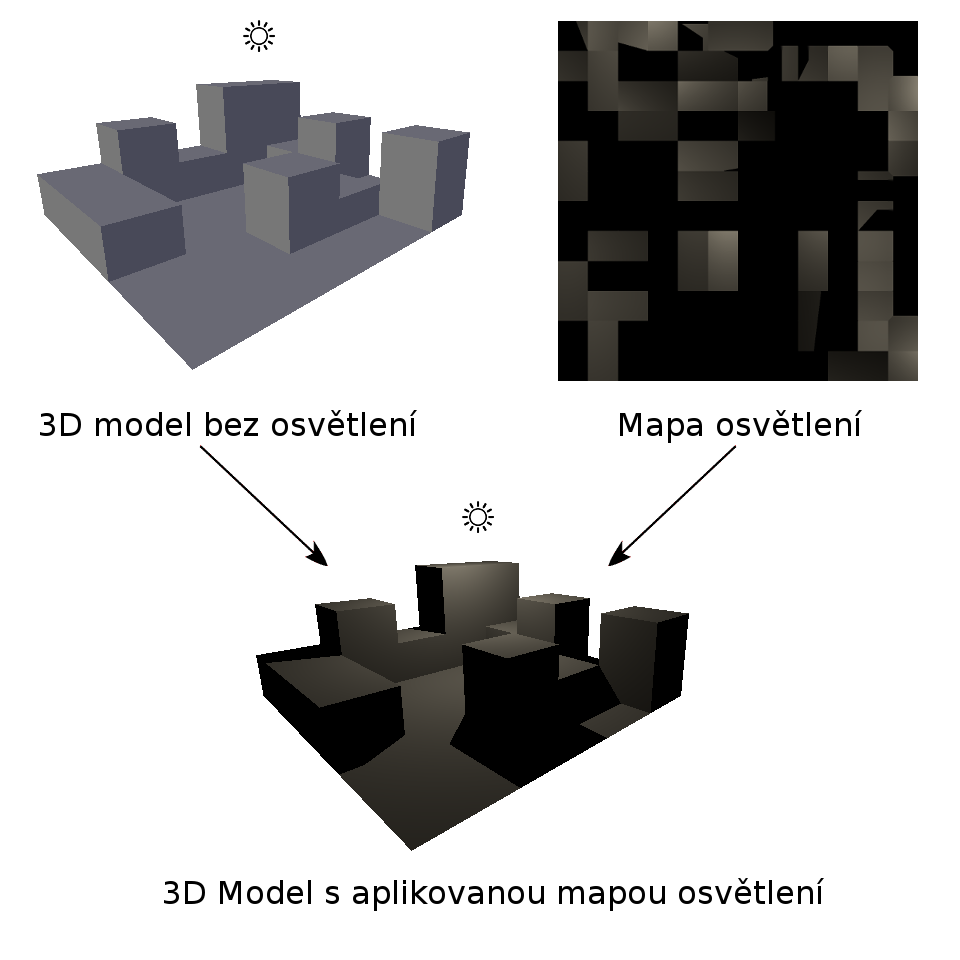
\includegraphics[width=100mm]{figures/lmapply.png}
\caption{Ukázka mapy osvětlení na jednoduchém 3D modelu}
\end{figure}
\end{center}

Aby bylo možné mapy osvětlení dynamicky aktualizovat, je potřeba mít do map rychlý zapisovací přístup. Rychlé zapisování do textur se v OpenGL realizuje pomocí Frame Buffer Objektu (FBO). Pro aktualizaci musíme mít předpočítanou tzv. záplatu. Záplatou se rozumí menší textura, která se přidá do současné osvětlovací mapy. Přidáním záplaty lze tedy přidat do scény další světlo, které máme předpočítané. Záplata jde z FBO opět odebrat (provede se odečet stejné záplaty).

Protože uchovávání záplat v paměti by bylo příliš paměťově náročné, jsou uloženy\linebreak ve vektorové podobě přímo na GPU pomocí Vertex Buffer Objektu (VBO). 
\newpage

\begin{center}
\begin{figure}[h!]
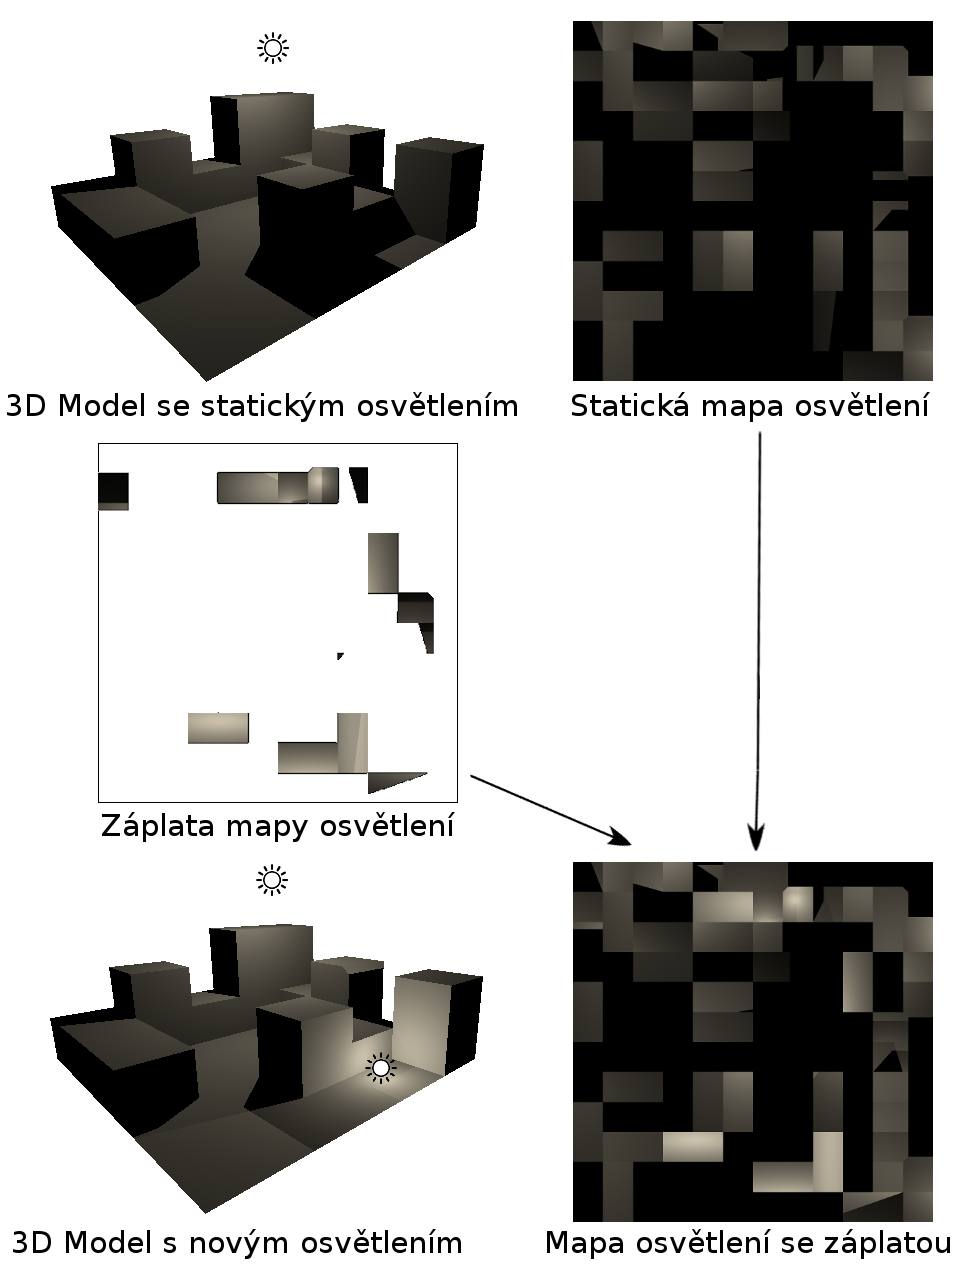
\includegraphics[width=110mm]{figures/lmupdate.png}
\caption{Ukázka aktualizace map osvětlení na jednoduchém 3D modelu}
\end{figure}
\end{center}

\subsection{Statické osvětlení s dynamickými objekty ve scéně}
Při použití dynamických objektů ve scéně se statickém osvětlením vznikají dva základní problémy. Prvním problém je, že dynamické objekty mají jiné osvětlení než statická scéna\linebreak a to vypadá velice nepřirozeně. Druhým problémem je, že pokud dynamický objekt zastíní zdroj světla, tak nevznikne stín na statických objektech.

Oba problémy lze vyřešit jen částečně. V prvním případě lze přečíst informaci o intenzitě osvětlení z nejbližšího bodu na statickém objektu a tuto intenzitu aplikovat na dynamický objekt. V druhém případě při vykreslování jednotlivých pixelů lze zjistit, zda se v okolí vykreslovaného bodu nenachází dynamický objekt a tím aproximačně zjistit zda byl vykreslovaný bod zastíněn.
\newpage

\section{Cílová platforma Android}
Platforma Android je postavena na Linuxovém jádře a využívá knihovny, které bývají součástí unixových systémů. Od klasického desktopového Linuxu se odlišuje hlavně v tom, že jako hlavní programovací jazyk využívá Javu. Pomocí Javy je naprogramováno celé Android API, které zprostředkovává téměř veškeré služby systému.

Na Androidu je téměř nemožné spustit C/C++ program přímo. Standardně se to řeší tak, že se vytvoří z programu knihovna, kterou spustí kód napsaný v Javě. Pak je nutné veškeré vstupy/výstupy obsluhovat v jazyce Java a to velice komplikuje portování programů z desktopového Linuxu na Android. Výjimku tvoří OpenGL, které umožňuje vykreslovat\linebreak na displej přímo z C/C++ kódu.

\begin{center}
\begin{figure}[h!]
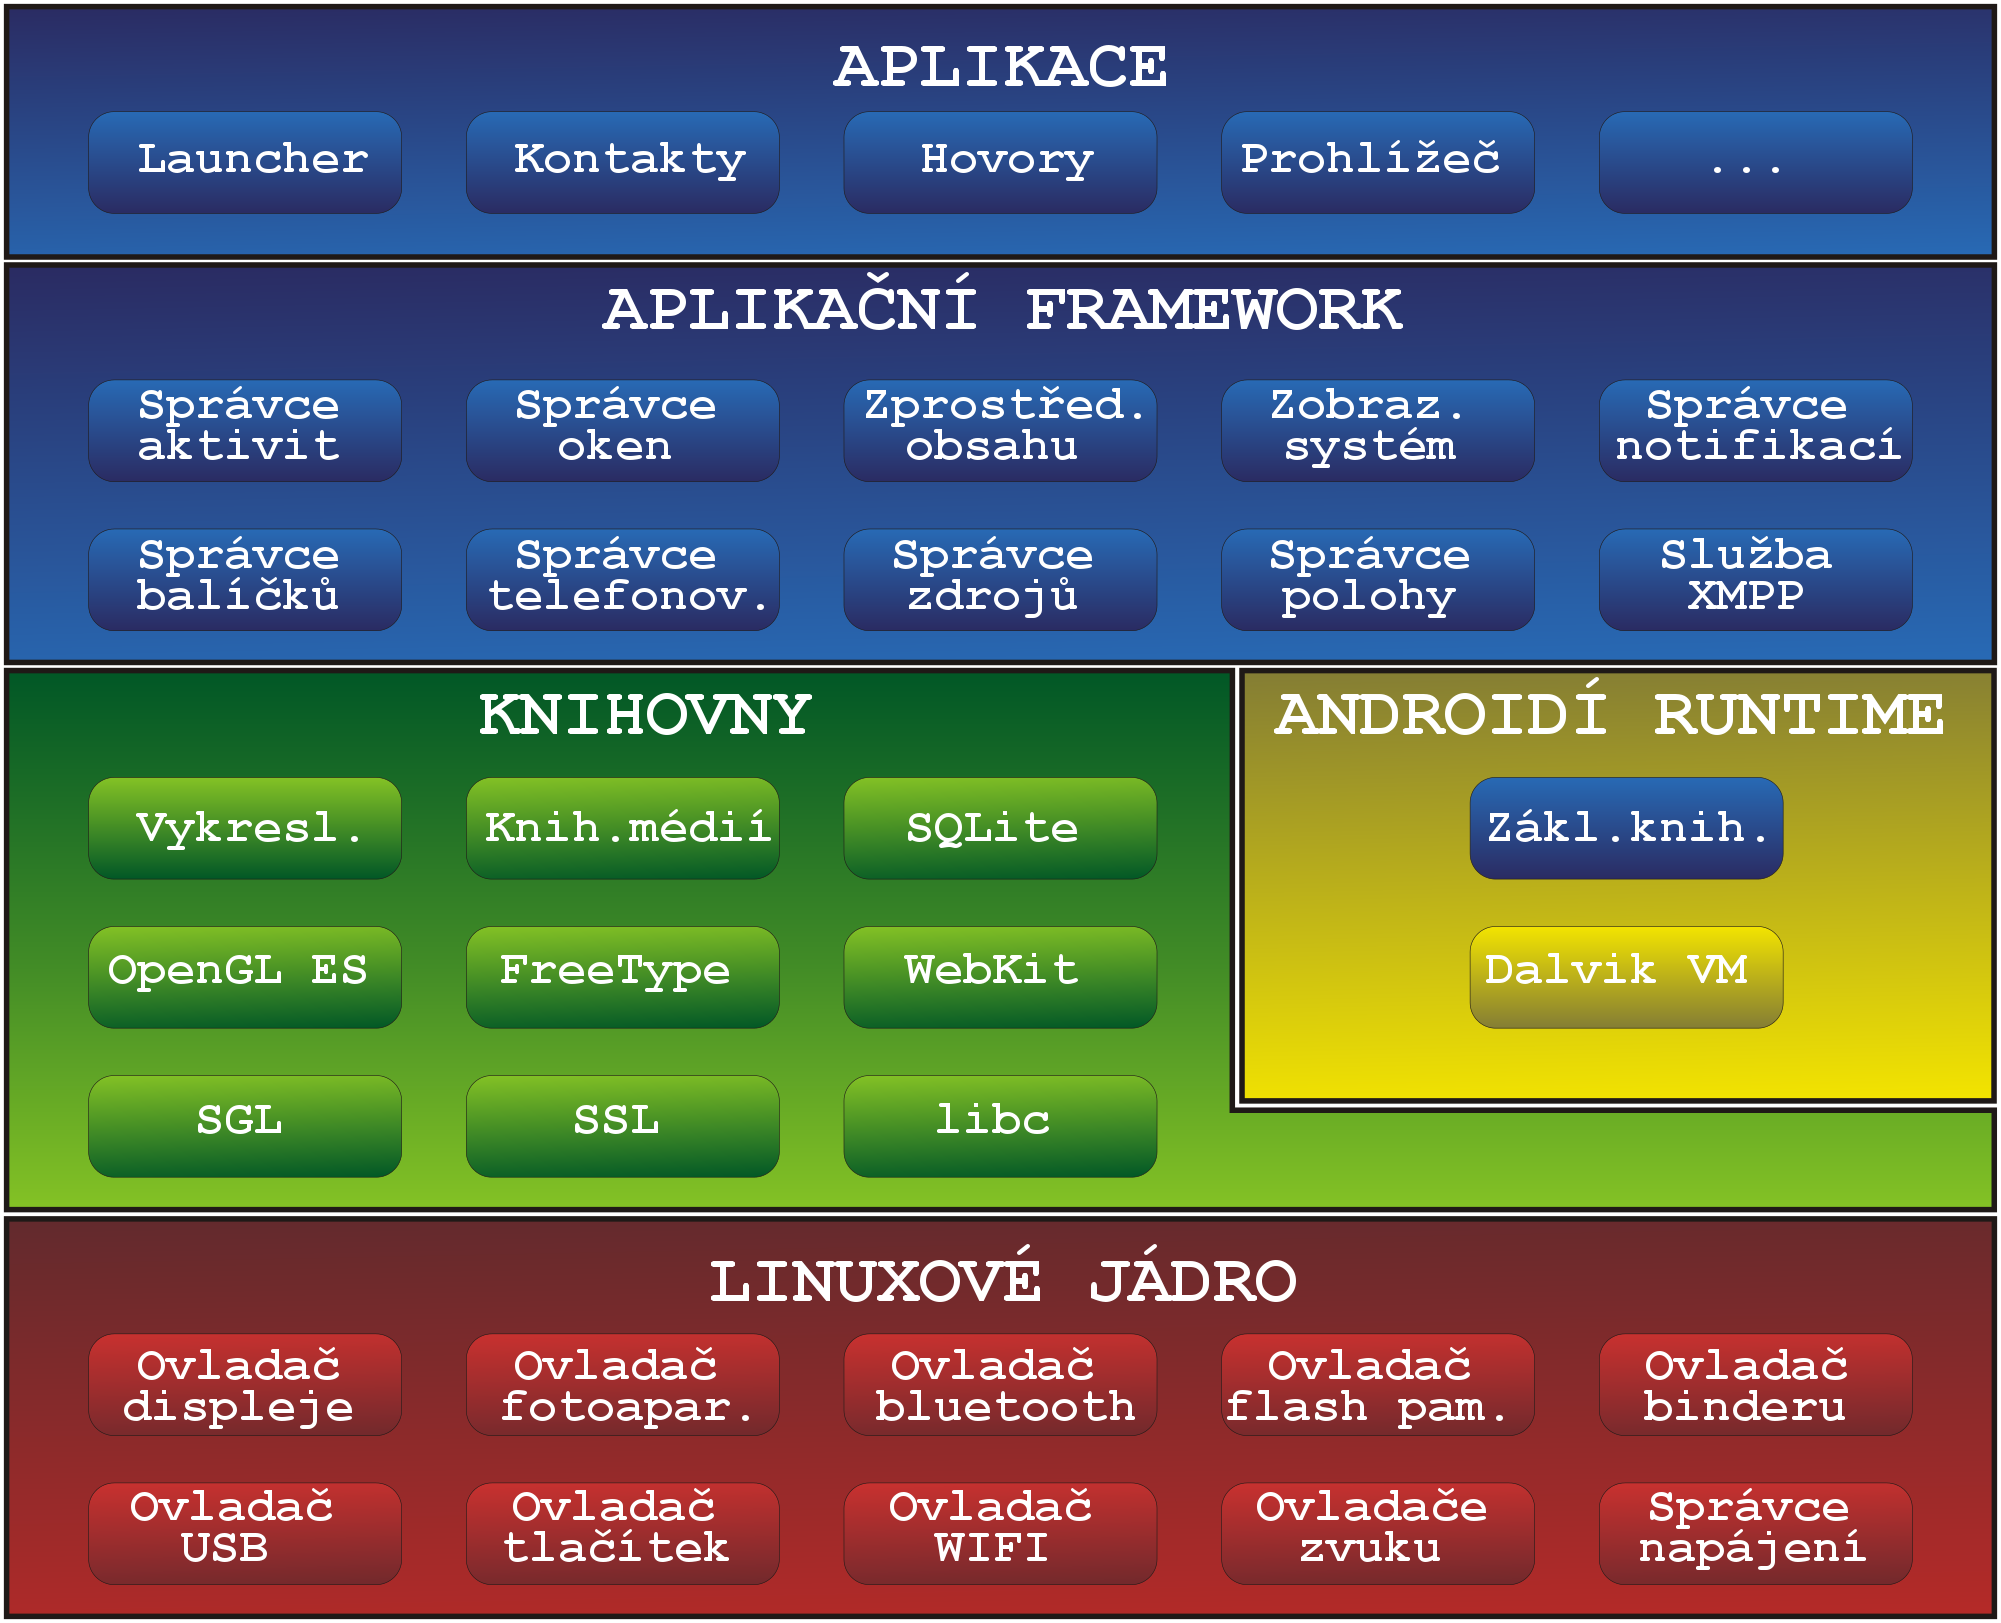
\includegraphics[width=120mm]{figures/android.png}
\caption{Komponenty platformy Android, komponenty vyznačené modrou barvou jsou napsané v jazyce Java, žlutou barvou je virtuální stroj, který umožňuje běh Java aplikací, zelenou barvou jsou C/C++ knihovny a červenou je Linuxové jádro}
\end{figure}
\end{center}

Pro platformu Android existuje nepřeberné množství aplikací a toho začínají využívat ostatní platformy. V současné době platformy BlackBerry a Jolla umožňují spouštět Android aplikace, dále existuje platforma NokiaX, která je postavena přímo na operačním systému Android.

\section{Existující implementace}

Rešerši existujících implementací jsem zaměřil na dvě různé kategorie. První kategorie jsou implementace pro PC, kde je nejčastěji řešeno nepřímé osvětlení, které by na mobilních zařízeních zatím použít nešlo. Druhá kategorie jsou závodní simulátory s noční jízdou pro platformu Android. V této kategorii bývají nejčastěji použity techniky jako v této práci.

\subsection{Projekty zabývající se vykreslování noční scény}

V této sekci jsem vybral co nejrealističtější implementace, ke kterým existuje nějaký článek o tom, jak bylo výsledku dosaženo. Existuje sice několik implementací, které vypadají ještě více realističtěji. To jsou ale většinou komerční produkty, které nesdílejí ostatním, jakým způsobem byla implementace realizována.

\subsubsection{Proceduralní modelování města a osvětlení nočního města}
Tato implementace je z roku 1999 a zabývá se proceduálním modelováním města (konkrétně Bostonu) a následně jej vykresluje pomocí sledování paprsku za využití algoritmu Monte Carlo. Implementace pochopitelně neběží v reálném čase. Výsledek je při detailním záběru po grafické stránce velice realistický. Vytknul bych jen, že reflektory vozidla osvítí pouze blízké okolí. Při záběru na město z výšky výsledek nebudí tolik realistický dojem jako při detailním záběru.

\begin{center}
\begin{figure}[h!]
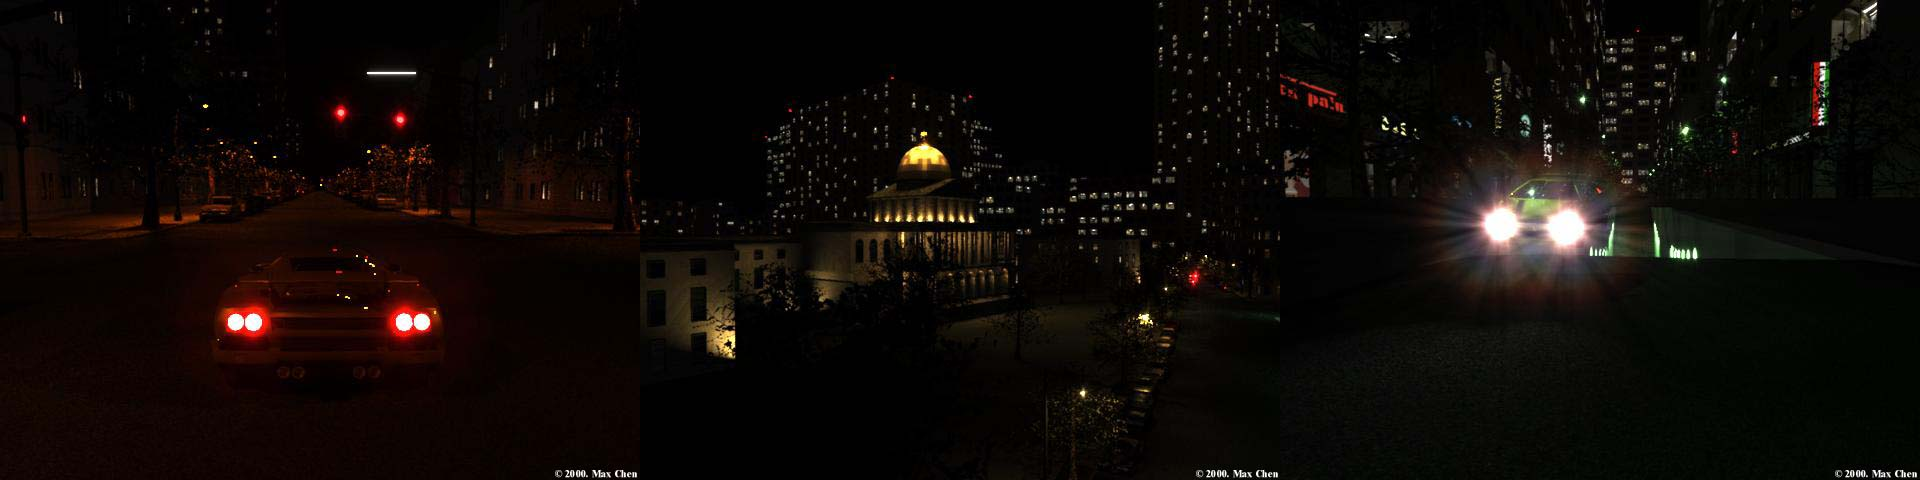
\includegraphics[width=150mm]{figures/NR.png}
\caption{Ukázka nočního renderingu}
\end{figure}
\end{center}
\newpage

\subsubsection{Imperfektní stínové mapy pro výpočet nepřímého osvětlení}
Tato implementace, představená roku 2008, se nezabývá přímo noční scénou, zabývá se nepřímým osvětlením, které s noční scénou souvisí. Implementace běží v reálném čase a její výsledky jsou srovnatelné se snímky, které se vykreslují několik hodin.

V této implementaci se nevyužívá předpočtených dat. Využívá se zde virtuálních bodových světel (VPL), která simulují odrazy světla. Z každého VPL se vytvoří stínová mapa o malém rozlišením a při vykreslování výsledné scény se vyhodnocuje viditelnost ze všech VPL.

Implementace podporuje více typů zdrojů světla, včetně plošných. Nemá problémy\linebreak s barevným světlem ani s kaustiky.

\begin{center}
\begin{figure}[h!]
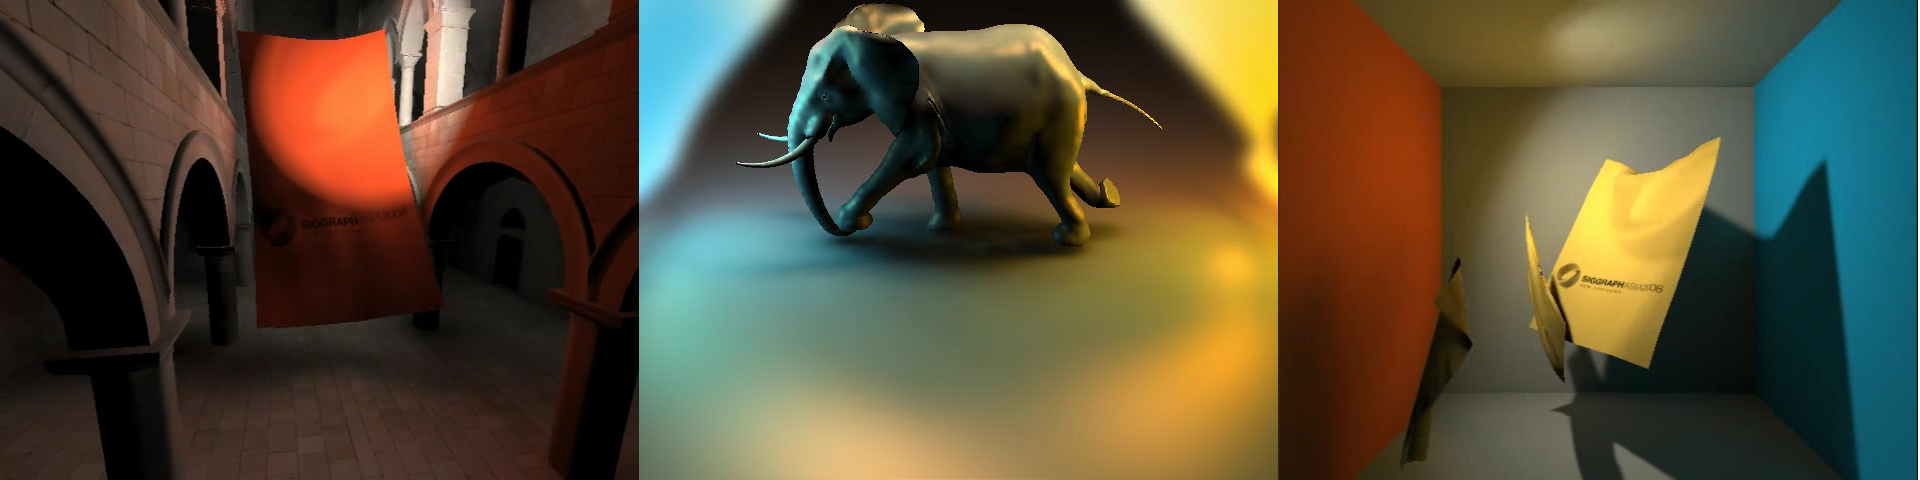
\includegraphics[width=150mm]{figures/ISM.png}
\caption{Ukázka výsledků techniky imperfektních stínových map pro efektivní výpočet nepřímého osvětlení}
\end{figure}
\end{center}

\subsection{Závodní simulátory s noční scénou pro platformu Android}
V této sekci jsem vyhledával i implementace, u kterých není uvedeno, jak bylo výsledků dosaženo. Je to z důvodu malého počtu implementací odpovídající dané kategorii.

\subsubsection{Asphalt Urban od Gameloftu}
Asphalt Urban je série mobilních závodních simulátorů, jejíchž první díl byl publikován spolu s herním smartphonem Nokia N-Gage. Jedná se o úspěšnou sérii, která přitahuje hráče všech možných platforem.

Zmíním 7.díl ze série Asphalt Urban, který osobě považuji za nejúspěšnější díl. Osvětlení z pouličních lamp je součástí textur, reflektor vozidla je tvořen zřejmě pomocí projektivní textury. Povrch zrcadlově odráží 3D objekty. Po bližším zkoumání lze zjistit, že některé tyto odražené objekty jsou odlišné. Domnívám se, že zde byl použit duplicitní objekt.

Další díl ze série Asphalt Urban už odlesky řeší lépe. Odráží se hlavně světla a odlesk je lépe přizpůsoben povrchu. Vzniká zde dojem mokré silnice. Dochází i k rozmazání brzdových světel. Osvětlení od lamp je opět řešeno texturou. Nepříjemnou změnou je absence reflektoru vozidla a přidání rušivého chvění kamery během jízdy.

\subsubsection{Need for Speed Most Wanted od EA Games a Firemonkeys}
Simulátor, který je spíše známý z PC, na mobilním trhu takový úspěch nemá. Od PC verze je velice odlišný, ale rozhodně se nejedná o nějakou lacinou napodobeninu. Jedná se o první závodní simulátor pro mobilní zařízení, který disponuje modelem ničení vozidla (je možné vozidlo poškrábat, rozbít mu okna apod).

Oproti Asphalt 8 má navíc efekt Depth-of-field. To znamená, že vzdálené modely jsou rozmazané a zabarveny do barvy pozadí. Tento efekt vytváří přijemný mlhovitý dpjem. Jinak bych řekl, že tyto dva simulátory jsou si sobě velice podobné. Na stejném enginu funguje\linebreak i známý simulátor Real Racing 3, který ale noční jízdu nemá.

\subsubsection{GT Racing 2 od Gameloftu}
Úspěšným závodním simulátorem je v současné době GT Racing 2, je to hlavně díky jeho zpracování. Jako jediný z uvedených simulátorů má při noční jízdě nízké ambientní osvětlení a scéna je osvětlena hlavně reflektorem vozidla.

Nejsem si jist, zda osvětlení lampami je přímo součástí textur nebo jestli jsou zde použity mapy osvětlení.

\subsubsection{Sports Car Challenge od Fishlabs}
Asi nejdetailnější model vozidla má právě Sports Car Challenge. Vývojář spolupracuje s předními výrobci automobilů a to se odrazilo právě na modelech vozidel. Modely jsou realistické a to včetně interiérů.

Projekt trpí slabší kompatibilitou s mobilními zařízeními, i když náročnost enginu je nízká. Co se týká noční jízdy, je realizována stejnými technikami jako denní jízda. Jsou zde použity pouze tmavé textury a halo efekt pouličních lamp.

\subsubsection{Track Racing od vývojáře Soulkey}
I když tento projekt není závodní simulátor s noční jízdou, zmiňuji ho hlavně kvůli ovládání. Jedná se o neoficiální remake hry Trackmania známé z PC. Projekt běží na Unity3D enginu a je dostupný na mnoha platformách, nedá se ale stáhnout přímo z Marketu či Storu.

U výše uvedených simulátorů vozidlo automaticky zrychluje a u některých i samo brzdí. Hráč nemá tedy nad vozidlem takovou kontrolu. V případě Track Racing má hráč nad vozidlem plnou kontrolu a zážitek ze hry se dá srovnat se zážitkem z původní PC hry.
\newpage

\begin{center}
\begin{figure}[h!]
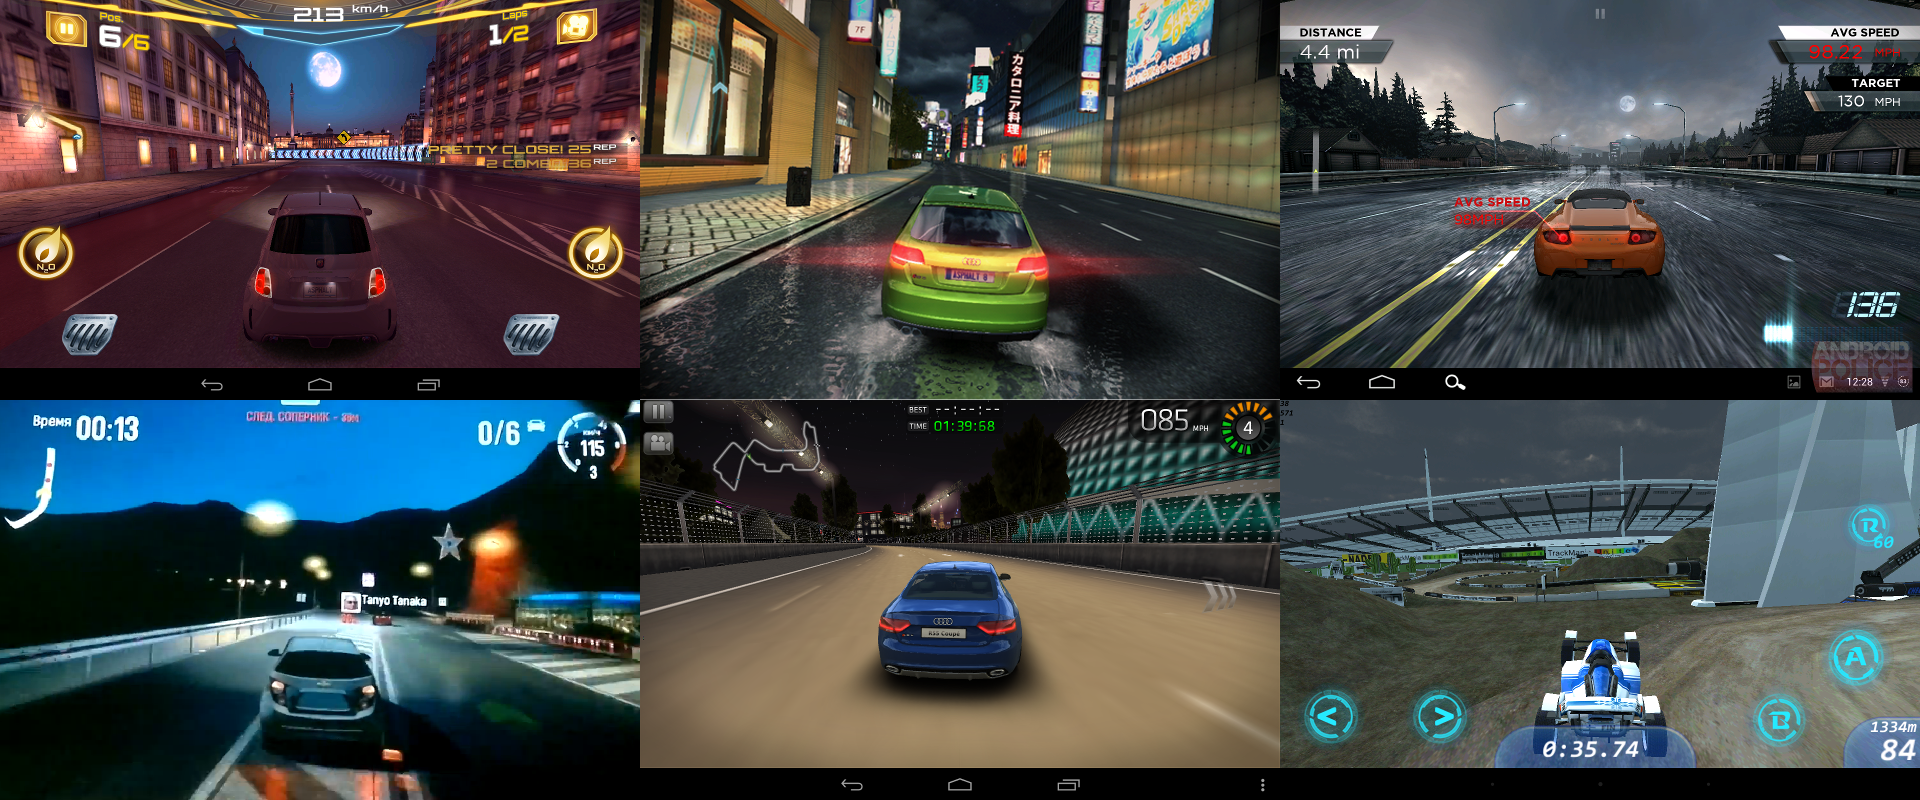
\includegraphics[width=150mm]{figures/games.png}
\caption{Ukázka závodních simulátorů s noční scénou pro platformu Android, první řada zleva: Asphalt 7, Asphalt 8, Need for Speed Most Wanted, druhá řáda zleva: GT Racing 2, Sports Car Challenge, Track Racing}
\end{figure}
\end{center}

%*****************************************************************************
\chapter{Teoretická část}

\section{Osvětlovací model}
Existuje několik osvětlovacích modelů, asi nejpoužívanější lokální osvětlovací model je Phongův. Phongův model se skládá ze tří typů osvětlení:
\begin{itemize}
\item ambientní osvětlení - nahrazuje nepřímé osvětlení konstantní hodnotou osvětlení
\item difúzní osvětlení - osvětlení nezávislé na pohledu kamery, Odpovídá ideálně matnému povrchu
\item spekulární osvětlení - osvětlení závislé na pohledu kamery, odpovídá ideálně odrazivému tělesu povrchy
\end{itemize}

Jak je patrné z obrázku 3.1, výsledná intenzita povrchu $I$ je součtem ambientní složky ($I_a$), difúzní složky ($I_d$) a spekulární složky ($I_s$):
\begin{center}
$I = I_a + I_d + I_s$
\end{center}

\begin{center}
\begin{figure}[h!]
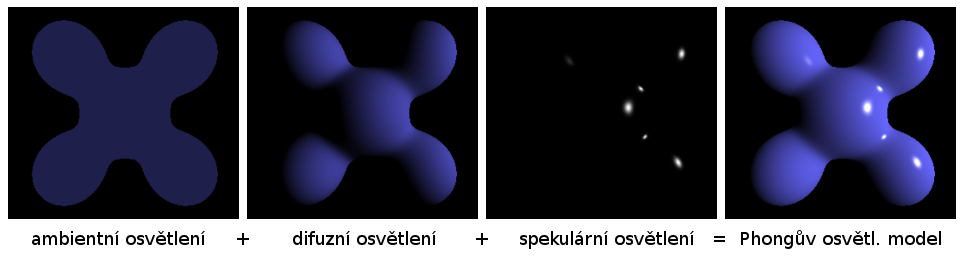
\includegraphics[width=150mm]{figures/phong.png}
\caption{Phongův osvětlovací model}
\end{figure}
\end{center}

Všesměrové osvětlení je ve Phongovo osvětlovacím modelu konstantní pro celou scénu\linebreak a říká se jí ambientní osvětlení $I_a$. Výsledná intenzita se spočte jako součin konstant barvy ambientního světla $C_a$, koeficientem ambientního odrazu $k_a$ a barvou povrchu $C_d$, která je shodná i pro difúzní složku:
\begin{center}
$I_a = C_a \cdot k_a \cdot C_d$
\end{center}

Difúzní složka odpovídá ideálně matnému (Lambertovskému) povrchu a závisí na úhlu $\alpha$ mezi vektory $\vec{L}$ a $\vec{N}$.
\begin{center}
\begin{figure}[h!]
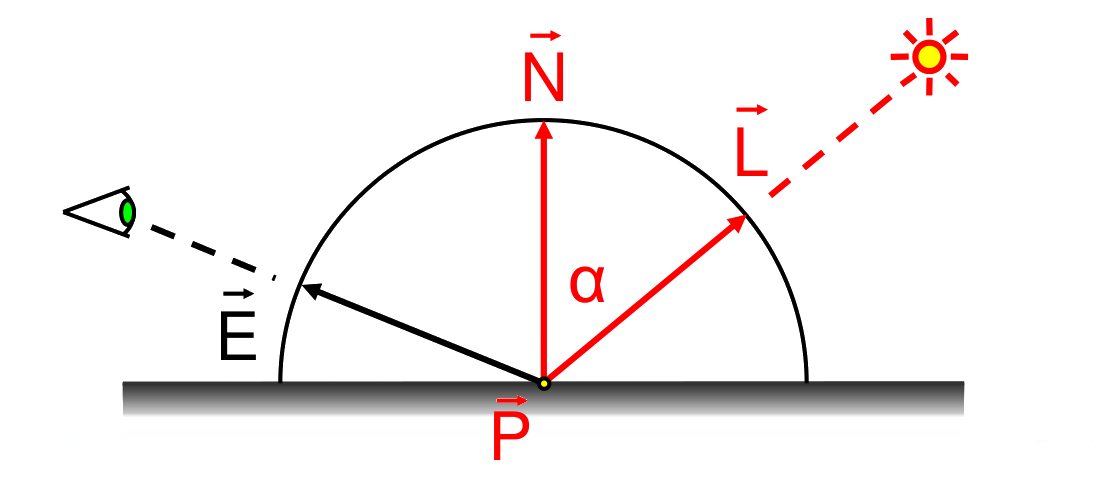
\includegraphics[width=60mm]{figures/phongD.png}
\caption{Difúzní osvětlení, $\vec{L}$ je normalizovaný směr světla, $\vec{N}$ je normalizovaná normála povrchu, $\alpha$ je úhel, který tyto vektory svírají, $\vec{E}$ je normalizovaný směr pohledu kamery (eye vektor) a $P$ je bod na povrchu tělesa}
\end{figure}
\end{center}
Intenzitu difúzní složky lze vyjádřit následovně:
\begin{center}
$I_d = C_l \cdot k_d \cdot C_d \cdot cos(\alpha)$
\end{center}
Kde $C_l$ je barva světla, $k_d$ koeficient difúzního odrazu, $C_d$ barva povrchu a pro úhel $\alpha$ platí, že $cos(\alpha) = \vec{L} \cdot \vec{N}$. Po dosazení tedy získáme výsledný výraz:
\begin{center}
$I_d = C_l \cdot k_d \cdot C_d \cdot (\vec{L} \cdot \vec{N})$
\end{center}
\bigskip

Spekulární (zrcadlová) složka odpovídá ideálně odrazivému tělesu a závisí na úhlu $\beta$ mezi vektory $\vec{E}$ a $\vec{R}$. 
\begin{center}
\begin{figure}[h!]
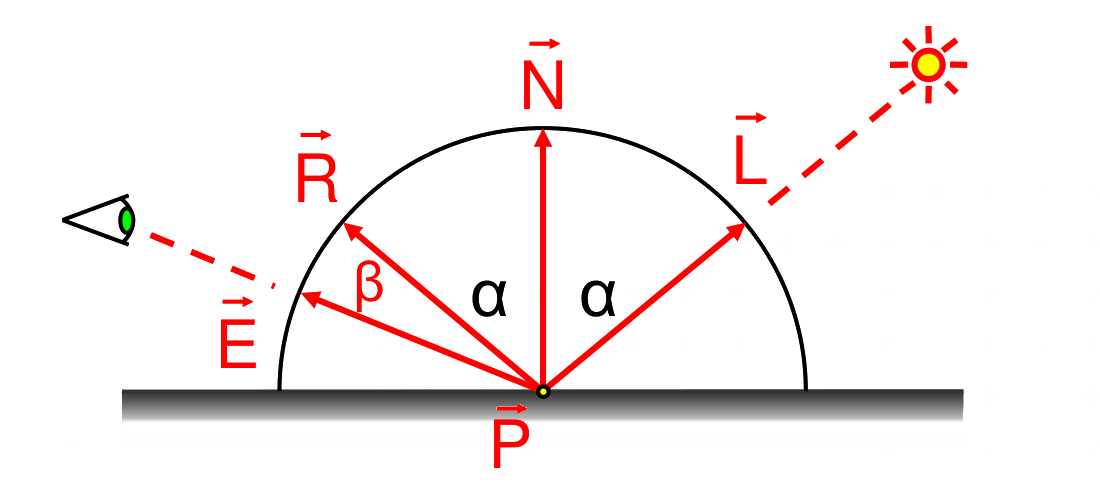
\includegraphics[width=60mm]{figures/phongS.png}
\caption{Spekulární osvětlení, $\vec{L}$ je normalizovaný směr světla, $\vec{N}$ je normalizovaná normála povrchu, $\alpha$ je úhel, který tyto vektory svírají, $\vec{E}$ je normalizovaný směr pohledu kamery (eye vektor), $\vec{R}$ je normalizovaný směr odrazu světla, $\beta$ je ůhel, který svírají vektory $\vec{E}$, $\vec{R}$ a $P$ je bod na povrchu tělesa}
\end{figure}
\end{center}

Intenzitu spekulární složky lze vyjádřit následovně:
\begin{center}
$I_s = C_l \cdot k_s \cdot C_s \cdot cos^h(\beta)$
\end{center}
Kde $C_l$ je barva světla, $k_s$ koeficient spekulárního odrazu, $C_s$ barva lesklého povrchu, která většinou bývá bílá, $h$ je ostrost odrazu a pro úhel $\beta$ platí, že $cos(\beta) = \vec{E} \cdot \vec{R}$. Po dosazení tedy získáme výsledný výraz:
\begin{center}
$I_s = C_l \cdot k_s \cdot C_s \cdot (\vec{E} \cdot \vec{R})^h$
\end{center}

\subsection{Výpočet osvětlení}

\subsection{Výpočet stínů v reálném čase}

\subsection{Spekulární složka osvětlovací modelu}

\section{Předvypočítané osvětlení}
Předvypočítané osvětlení je z hlediska vykreslování poměrně jednoduchá technika. Pouze se aplikuje další textura či textury, které mají vlastní texturovací souřadnice a nesou\linebreak v sobě informaci o osvětlení jednotlivých trojúhelníků. Těmto texturám se říká mapy osvětlení a dalo by se říct, že se jedná o techniku, která rozšiřuje techniku předvypočítaných stínů.

Z hlediska generování těchto textur je tato technika náročnější než výsledné vykreslování, skládá se z několika kroků. V prvním kroku je třeba vytvořit texturovací souřadnice pro jednotlivé trojúhelníky.

\subsection{Vytvoření texturovacích souřadnic}
TODO: přepsat
Jeden z velmi efektivních algoritmů řešící problematiku vytváření texturovacích souřadnic je Packing Lightmaps \cite{Scott02}. Za využití datové struktury kD stromu, která u tohoto algoritmu reprezentuje rozložení geometrie v mapě osvětlení, je možné řešit rozložení pro obdélníky. Aby bylo možné pracovat s trojúhelníky, je nutné algoritmus rozšířit.

Práci s trojúhelníky lze realizovat tak, že vždy dva trojúhelníky spolu vytvoří jeden obdélník. Nejdříve se provede drobná deformace tak, aby všechny trojúhelníky byly pravoúhlé(je nutné hlídat, aby se nesnižoval počet texelů připadající na daný trojúhelník). Poté už stačí trojúhelníky vhodně spárovat(vytvořit z nich obdélníky) a je možné spustit původní algoritmus.

Jak je kD strom použit je vidět na následujícím obrázku. V uzlech jsou provedeny řezy, kterými se rozděluje rovina, v listech jsou pak jednotlivé objekty.
TODO: popis algoritmu

\begin{center}
\begin{figure}[h!]
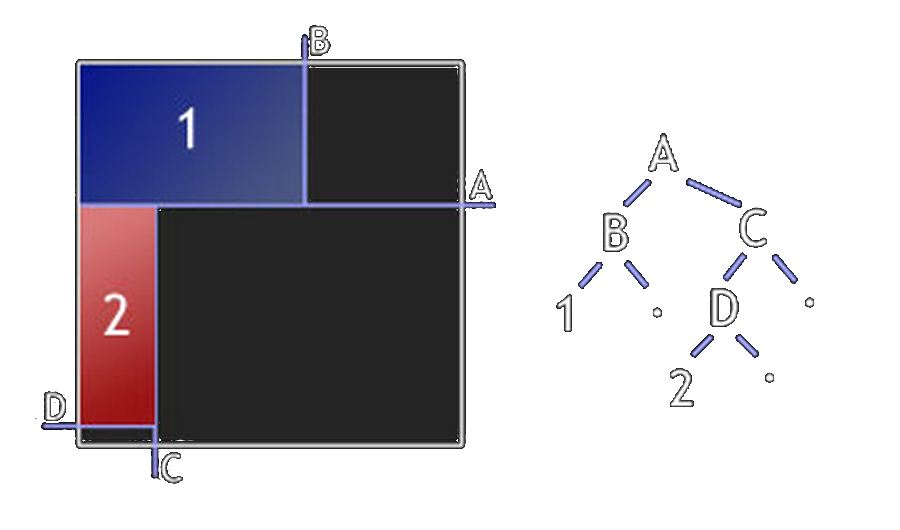
\includegraphics[width=120mm]{figures/packingLM.png}
\caption{kD strom v metodě Packing Lightmaps}
\floatfoot{Zdroj: \cite{Scott02}}
\end{figure}
\end{center}
\newpage

\subsection{Generování map osvětlení}
Generování map osvětlení lze provádět pomocí rasterizace nebo vrhání paprsku. Vrhání paprsku je v porovnání s rasterizací daleko složitější metoda. V rámci předmětu softwarový projekt se zabývám pouze rasterizací.

Generování se provádí pomocí standardního rasterizačního řetezce. Geometrie se netransformuje do souřadnic kamery, ale do souřadnic map osvětlení. Otexturovanou geometrii do souřadnic mapy osvětlení můžete vidět na obrázku 3.2.
\begin{center}
\begin{figure}[h!]
\includegraphics[width=70mm]{figures/LM-vse.png}
\caption{Model města transformován do souřadnic mapy osvětlení}
\end{figure}
\end{center}
\newpage

Dále je potřeba vyfiltrovat objekty, které nejsou viditelné. K tomu slouží stínová mapa. Stínová mapa je textura, která v sobě má uloženou vzdálenost od světla pro velké množství bodů. Při vykreslování se spočítá souřadnice bodu ve stínové mapě, z toho se získá vzdálenost bodu od světla. Porovnáním vzdálenosti od světla vykreslovaného bodu se zjistí, zda je bod osvětlený daným světlem. Viz obrázek níže.
\begin{center}
\begin{figure}[h!]
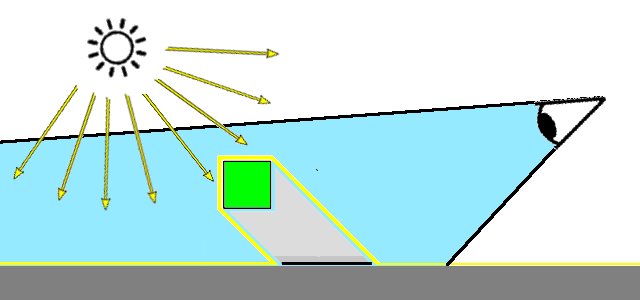
\includegraphics[width=100mm]{figures/shadowmapping.png}
\caption{Princip stínových map. Zdroj: \cite{Masserann11}}
\end{figure}
\end{center}

Tímto způsobem vyfiltrujeme neosvětlené objekty. Výsledek lze vylepšit využitím dalších technik jako je například útlum světla, PCF filtrování a další. TODO: akumulace více světel, přepsat

\subsection{Oprava chyby sousedících trojúhelníků}
Pokud bychom použili přímo souřadnice získané metodou Packing Lightmaps, vznikly by ve výsledné scéně chyby(buď v důsledku zaokrouhlování souřadnic nebo v případě lineárního filtrování vlivem sousedních texelů). Je proto nutné už při generování map osvětlení souřadnice posunout nepatrně směrem ke středu každého trojúhelníku. Po dokončení generování map osvětlení se provede postprocesing, který doplní mezery v mapách osvětlení vždy nejbližší možnou hodnotou.


\section{Odlesky povrchů}
Odlesky dodávají scéně lepší vzhled, dodávají dojem buď kovového nebo mokrého povrchu. V rasterizačním řetězci jsou odlesky drobet problematické, protože grafická karta vždy zpracovává pouze aktuální geometrii a nemá informaci o okolí.

Standardně se odlesk realizuje dalším průchodem, ve kterém se vykreslí okolí do textury a tato textura se pak aplikuje na model s odleskem. U menších objektů jako je třeba auto se vykreslí okolí ve formě cubemapy(krychle, která má na svých stěnách obrazy z okolí objektu). Cubemapa se následně \uv{nalepí} na objekt a tím se získá lesklý povrch.

V případě rovných povrchů je nutné použít jiný přístup, scéna se vykreslí do textury z pohledu, který je na obrázku 3.4 označen jako P'. Pohled snímá objekty jakoby z povrchu(všechny objekty pod povrchem je třeba vyfiltrovat). Při vykreslování na obrazovku se spočítá pozice daného pixelu povrchu ve vykreslené textuře a z té se aplikuje barva pixelu.

\begin{center}
\begin{figure}[h!]
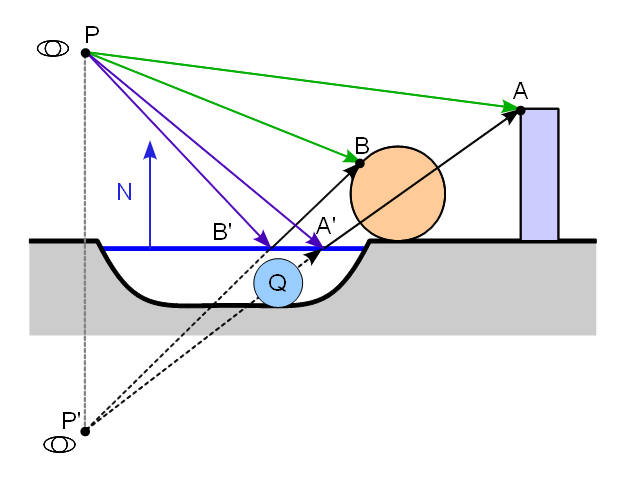
\includegraphics[width=80mm]{figures/reflection-diagram.png}
\caption{Diagram odrazu vodní hladiny}
\floatfoot{Zdroj: \cite{Kaplinski11}}
\end{figure}
\end{center}

\section{Screen-space přístup}
Základem screen-space přístupu je vykreslení scény do takzvaného geometry bufferu, který umožňuje na rozdíl od frame bufferu uložit daleko více informací o jednotlivých bodech. Dalšími informacemi typicky bývá normála, hloubka nebo informace k výpočtu spekulární složky světla. Geometry buffer je součástí OpenGL 4 a vyšší, ale některé poznatky o screen-space přístupu se dají použít i za pomocí staršího OpenGL.

Pomocí screen-space přístupu se dá implementovat mnoho efektů. V podstatě by bylo možné si v hlavním průchodu pouze vykreslit scénu pomocí velice jednoduchého shaderu\linebreak a osvětlovací model, případně další efekty, řešit až v průchodu pro screen-space data. Problém je, že screen-space průchod je typicky realizován pomocí jednoho shaderu a tedy musí být veškeré efekty a materiály implementovány v tomto shaderu.
\begin{center}
\begin{figure}[h!]
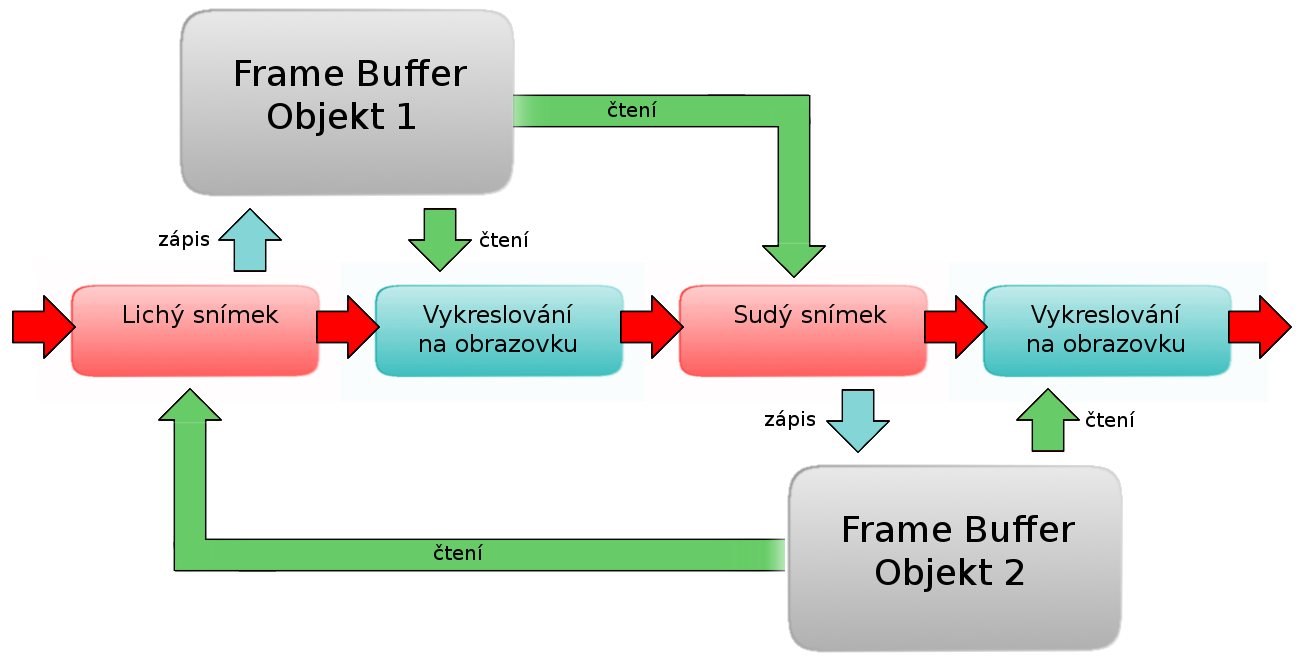
\includegraphics[width=70mm]{figures/screenspace.png}
\caption{Odraz objektů v screen-space přístupu}
\floatfoot{Zdroj: \cite{Pfaff12}}
\end{figure}
\end{center}

Problém nastává, pokud jsou potřeba číst informace, které jsou mimo rozmezí geometry bufferu. Tento případ nastává typicky při pokusu o vykreslení odrazivých ploch. Problém se často řeší absencí tohoto efektu pokud nejsou k dispozici potřebné informace. Aby absence nebyla tak rušivá, provádí se plynulý přechod mezi místy, kde efekt je a kde není(tedy jakoby na kraji geometry bufferu byl přechod do ztracena).

Odrazy zrcadel v budově se pochopitelně pomocí screen-space nedají řešit. Obecně lze říct, že odrazy pomocí screen-space lze realizovat jen u objektů, na které se kamera nebude dívat kolmo.

%*****************************************************************************
\chapter{Realizace}
Základním problémem realizace simulátoru na mobilních zařízení je jejich nízký výkon.
Uživatelé očekávají kvalitu grafiky srovnatelnou s počítačovou grafikou, nicméně mobilní zařízení zatím takového výkonu nedosahují.

\section{Předzpracování}

\subsection{Vytváření map osvětlení}

\subsubsection{Generování texturovacích souřadnic pro mapy osvětlení}

\subsubsection{Generování map osvětlení}

\subsection{Příprava dat pro dynamickou aktualizaci map osvětlení}

Ve fázi předzpracování se provede konverze 3D modelů do vlastního formátu, který bude umožňovat mít v sobě jak souřadnice standardních textur, tak i souřadnice v mapách osvětlení. Formát by měl zachovat veškeré informace o modelu. I když je třeba výsledný simulátor nevyužije, je dobré tyto informace ponechat pro případ dalšího vývoje. Formát by měl být schopen uložit některé další informace o materiálu a shaderu.

Plochu map osvětlení je nutné maximálně zaplnit z důvodu očekávané malé paměti vymezeny pro velké textury. Aby bylo možné určit nejvhodnější rozlišení těchto textur, je třeba umožnit jejich škálování.

Vykreslení hodnot do map osvětlení se provede pomocí OpenGL, bude zde řešena viditelnost (pomocí stínových map), vypočteno utlumení a výpočet difúzního odrazu světla.
TODO dopsat

\section{Simulátor}
Simulátor bude navržen tak, aby fungoval na X11-Linuxu a Androidu. Znamená to výběr multiplatformních knihoven nebo ve výjimečných případech rozdílná implementace pro jednotlivé platformy. K vykreslování jsem vybral OpenGLES 2.0 (jedná se o odlehčené OpenGL 3.0) a GLSL verze 1.0 (to zaručí maximální možnou kompatibilitu).

Fyzikální vlastnosti vozidel budou realizovány pomocí enginu Bullet Physics (tento engine používá mnoho známých firem zabývajících se vývojem mobilních her). Zvuk bude realizován na mobilních zařízeních pomocí Android API a na Linuxu pomocí knihovny FMOD API. Správce oken je na Androidu třeba doprogramovat, aby fungovalo dotykové ovládání a pozastavení simulátoru (např při hovoru). Na Linuxu bude použitý freeglut.

\section{Realizace na platformě Android}
Platforma Android je postavená na Linuxovém jádře a využívá mnohé komponenty\linebreak z projektu GNU, nicméně celé Android API je v jazyku Java. Android využívá svůj Java virtuální stroj Dalwik. Pomocí Android NDK(native development kit) je možné zkompilovat C/C++ kód jako knihovnu, kterou je možné zavolat z jazyku Java. Toto je prováděno pomocí JNI(Java native interface).

Snažší by bylo naprogramovat simulátor přímo v Javě, ale tím bych ztratil možnost portovat simulátor na další platformy, které virtuální stroj Dalwik nemají. Dále by byl problém s použitím fyzikálního engine, který je napsaný v jazyce C++. Musel bych napsat interface pro fyzikální engine, který by mi umožnil komunikaci mezi C++ a Java kódem.

\subsection{Problematika Android API}
Java native interface je rozhraní, které umožňuje spustit C++ kód z jazyku Java a obráceně. Nicméně komunikaci nelze realizovat nějak jednoduše a je proto vhodné tuto komunikaci minimalizovat.
\lstset{language=C++} 
\begin{lstlisting}[caption=Volání Java metody z jazyku C++]
jclass cl = env->FindClass(className);
jmethodID m = env->GetStaticMethodID(cl, methodName, paramFormat);
env->CallStaticVoidMethod(cl, m, id, volume);
\end{lstlisting}

Udělal jsem tedy rozhraní, které odpovídá handlerům knihovny freeglut. Tedy nahrazuji veškeré funkce této knihovny svou implementací. Knihovna implementuje správu oken, vstup klávesnice a myši a volání idle a display funkcí. Klávesnice a myš byla pochopitelně plně nahrazena dotykovým ovládáním, ale pokud do Android zařízení připojíme klávesnici nebo myš, bude plně funkční. Funkčnost myši zařizuje sám systém, klávesnice stačila namapovat.

\subsection{Využití vláken}
Většina zařízení, které dnes už spadají do střední třídy, je vybavena aspoň dvěma procesory, je proto vhodné rozdělit činnost do více vláken, aby bylo dosaženo maximálního výkonu. Třída GLSurfaceView, která umožňuje vykreslovat OpenGL scénu z C++ umožňuje volat OpenGL příkazy pouze z jednoho vlákna. Z tohoto důvodu jsem rozdělil kód na grafické\linebreak a negrafické vlákno.

V menu simulátoru se používá pouze grafické vlákno, negrafické vlákno je primárně použito pro fyzikální výpočty, které zařízení vytěžují nejvíce. Vlákna jsou synchronizovaná, aby nedocházelo k použití transformace vozidla z předešlého snímku(to by bylo velmi rušivé).

Dále provádím regulaci rychlosti simulátoru v závislosti na výkonu hardwaru. Ukázalo se, že je daleko příjemnější hru zpomalit, než aby docházelo k trhanému zobrazení. Problém je, že nelze zpomalovat rychlost simulátoru do nekonečna, proto je zde nastavena minimální hodnota, na kterou se může simulátor zpomalit. Je zde i horní limit, aby nedocházelo\linebreak k zrychlené jízdě a tedy i ke zvýšené spotřebě energie.

\subsection{Práce se soubory}
V Androidu se aplikace publikují v APK balíčku. Jedná se o ZIP soubor, který má nějakou danou strukturu. V Java kódu je možné na veškeré soubory uvnitř balíčku přistupovat,\linebreak v C++ tato možnost není. Někteří vývojáři toto řeší, že po prvním spuštění si aplikace stáhne ze serveru přídavná data a ty si uloží například na paměťovou kartu. Lze také rozbalit soubory z APK balíčku a s těma pak v C++ pracovat. To se moc nepoužívá, protože jsou potom data v zařízení dvakrát.

Další možnou variantou je přistupovat k APK balíčku jako k ZIP souboru. Knihovna libzip umožňuje zpracovávat data ze ZIP souboru jako kdyby byla uložena normálně na disku nebo na paměťové kartě. To má výhodu, že data jsou komprimovaná a zároveň přístupná. Tato varianta je tedy lepší než stahovat data ze serveru.

\section{Nahrazení víceprůchodových přístupů}
Při běhu jakéhokoliv simulátoru je největší zátěž mobilního hardware způsobena vykreslováním 3D scény, proto je nutné tuto část co nejvíce zefektivnit. Pro mnoho efektů se používají takzvané víceprůchodové přístupy(scéna se vykreslí víckrát z různých pohledů nebo pomocí různých shaderů), ale na mobilním zařízení je zatím z hlediska výkonu možné použít pouze jednoprůchodový přístup.

Abych částečně nahradil ve svém simulátoru víceprůchodový přístup, použil jsem screen-space přístup(to je obecně jakákoliv technika využívající data z pohledu kamery, jinými slovy máme pouze výsledný snímek a na něm provádíme další operace). V praxi se používá hlavně pro zrcadlové plochy. Potřeboval jsem přistupovat do aktuálně vykreslovaného snímku. To je ale problém, protože tento snímek není kompletní a kdybych vykresloval přímo do něj\linebreak a zároveň z něj četl způsobilo by to chyby ve výsledném obraze.

Řešením je vykreslování střídavě do dvou různých textur. To znamená, že při lichém snímku kreslím do textury 1 a čtu z textury 2. Při sudém snímku je tomu obráceně. Tímto způsobem získám přístup do vykreslené scény, sice s drobným zpožděním, ale při dostatečně rychlém vykreslování si toho uživatel nevšimne(za předpokladu, že textura bude použita\linebreak na efekty jako jsou odlesky nebo stíny).

\begin{figure}[h!]
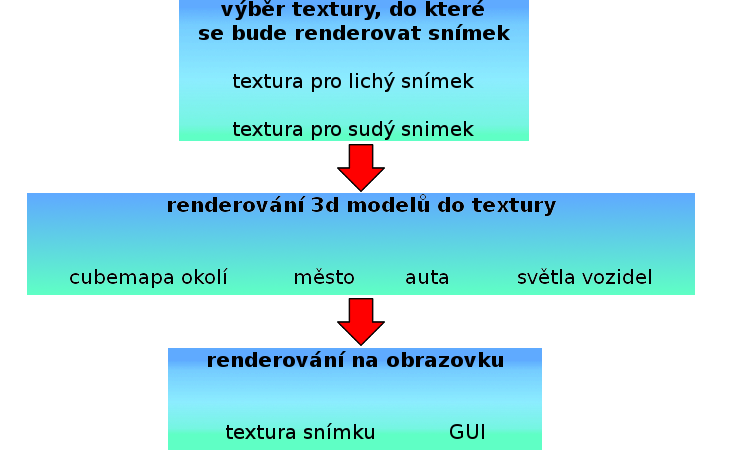
\includegraphics[width=150mm]{figures/render-schema.png}
\caption{Vykreslovací řetězec simulátoru}
\end{figure}

\subsection{Rozměr textur na OpenGL ES 2.0}
Verze OpenGL ES 2.0 neumožňuje používat obdélníkové textury. Textury musí být čtvercové a jejich strana musí být o velikosti mocniny 2.
Pro vykreslování do textury, která bude výsledně umístěna na obrazovku je tedy nutné zvolit vyšší rozlišení. Např. u tabletu Google Nexus 7 2012 s rozlišením 1280x720 se zvolí textura 2048x1024. To znamená, že by se ve výsledku vykreslilo víc než 2x více pixelů než je potřeba.

Není ale nutné vykreslovat do celé textury, pomocí příkazu \textit{glViewport} se dá nastavit část textury, do které má OpenGL vykreslovat a nedojde tedy k plýtvání výkonem(bude se plýtvat pouze pamětí).

Dále je možné zvolit nižší rozlišení viewportu než je rozlišení displeje. Mobilní zařízení obvykle disponují obrovskou hustotou pixelů a pokud zařízení nebude stíhat vykreslovat scénu v plném rozlišení, lze vykreslovat v rozlišení menším. U počítačových 3D her se také setkáváme s možností změnit rozlišení, tam řeší změnu přímo hardware displeje nebo jeho ovladač.

\subsection{Efekty pomocí screen-space přístupu}

Jedním z velmi rychlých efektů ve screen-space je \textbf{motion-blur}.
\lstset{language=GLSL} 
\begin{lstlisting}[caption=Motion blur fragment shader dle rychlosti vozidla]
uniform sampler2D color_texture, pFrm;
uniform float res, speed;
varying vec2 v_Coords;

void main() {
	//apply color texture
	gl_FragColor = texture2D(color_texture, v_Coords); 

	//apply motion blur
	gl_FragColor *= (1.0 - speed);
	gl_FragColor += speed * texture2D(pFrm, gl_FragCoord.xy * res);
}
\end{lstlisting}

Speed je rychlost vozidla od 0 do 1, pFrm je textura předchozího snímku a res je 1 / plné rozlišení textury(pro jednoduchost je použitý čtvercový rozměr textury).

Tento kód je použit přímo při renderování modelů, nikoliv při postprocesu. Výhodou je, že rozmaznutí se projeví po několik snímků za sebou pomocí jednoho čtení textury navíc. Nevýhodou je, že tento kód musí být vložen do každého shaderu vykreslující 3D model.
\bigskip

Dále je možné ve screen-space řešit \textbf{odlesky}. Existuje obecný(složitý) postup jak tyto odlesky vypočítat, který by mobilní hardware nezvládl. Problém jsem rozdělil podle typu ploch. Vzhledem k tomu, že v simulátoru dochází pouze k rotaci pohledu podle osy y(rotace yaw), je možné řešit pro odlesky pro různé směry normál zvlášť.

Například u vozovky stačí nalézt, kde vozovka končí, a podle toho obraz převrátit. Korektně to pro zatím z hlediska výkonu není možné vypočítat, proto dochází k velké nepřesnosti odlesku. Odhad zlomu je prováděn pomocí normály a pozice daného fragmentu, do kterého se odlesk započítává.

\begin{figure}[h!]
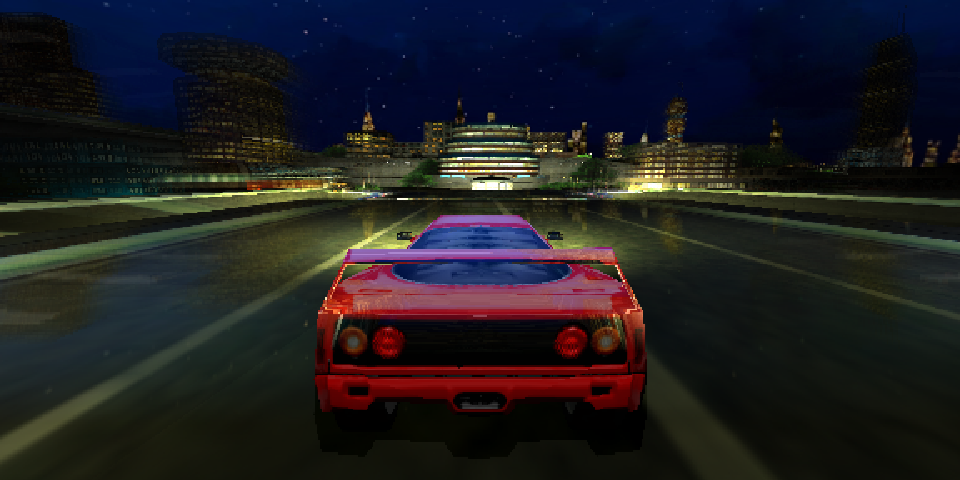
\includegraphics[width=150mm]{figures/reflect-horizont.png}
\caption{Odlesky na povrchu vozovky.}
\end{figure}
\bigskip

U vozidel se odlesk provádí pouze podle normály. Pro výpočet pozice odraženého obrazu se vezme střed vozidla a přičte se k němu normála vynásobena určitým faktorem(funguje pouze u vozidla, které uživatel ovládá).

\begin{figure}[h!]
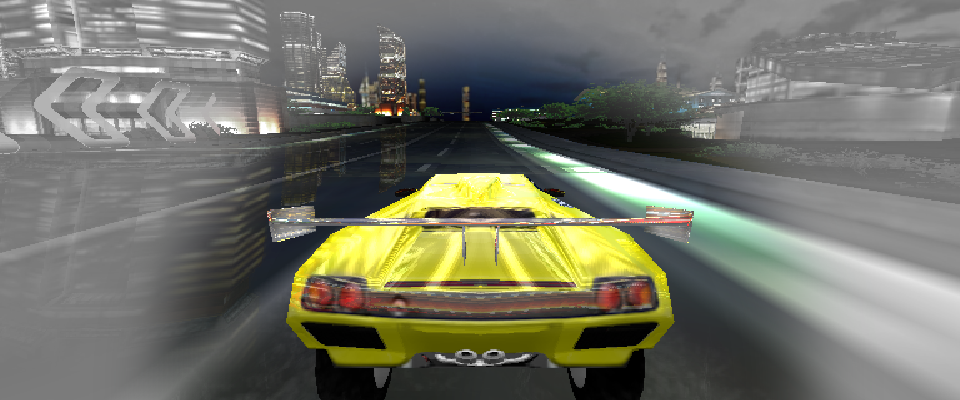
\includegraphics[width=150mm]{figures/reflect-car.png}
\caption{Odlesky na vozidle. Bílé plochy znázorňují pozice, ze kterých se čte barva odlesku.}
\end{figure}
\newpage

Pokud máme ve scéně \textbf{předvypočítané stíny}, je vhodné tyto statické stíny aplikovat\linebreak i \textbf{na dynamické objekty}. V případě vozidla lze přečíst intenzitu osvětlení z některých bodů na silnici pod vozidlem. Intenzitu osvětlení lze jednoduše ukládat do alfa kanálu textury,\linebreak ve které se nachází aktuální scéna.

Zde vzniká problém s barevným světlem. Jsou zde dvě možnosti řešení. Prvním je přidání další textury, ve kterém by byla barevná intenzita světla(tím by došlo ke zvýšení náročnosti na hardware a ke zvýšení paměťové náročnosti). Druhým možným řešením je omezit barevná světla do nějaké sytosti(pokud se slabě zabarvené světlo aplikuje jako bílé, není to tolik rušivé).

\section{Předvypočítané osvětlení}

Předvypočítané osvětlení umožňuje velmi rychle zobrazovat stínování a stíny na statických objektech. Problémem je, že je potřeba aplikovat tento efekt i na dynamických objektech. Úroveň osvětlení lze přečíst z nejbližšího statického objektu, tedy za předpokladu, že budeme mít tuto hodnotu někde k dispozici. Tuto hodnotu lze mít uloženou v alfa kanálu aktuálního snímku a jen jí přečíst před tím, než se vykreslí dynamické objekty.

\begin{figure}[h!]
\begin{center}
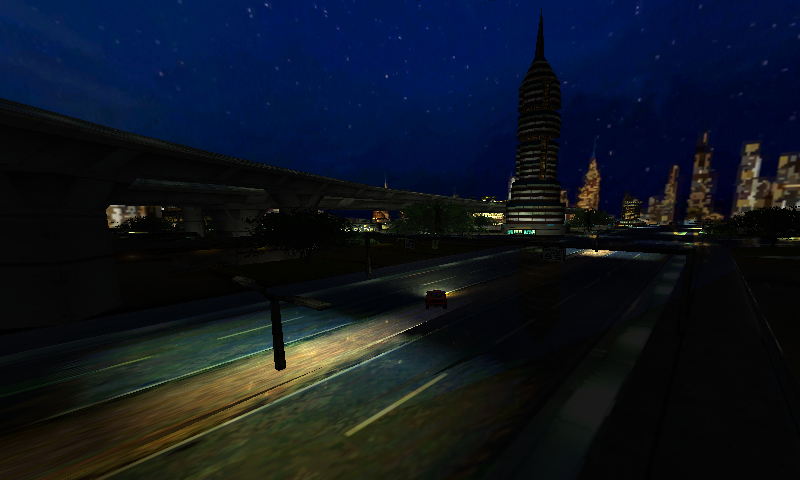
\includegraphics[width=110mm]{figures/lamps.png}
\caption{Scéna s aplikovanými mapami osvětlení lamp}
\end{center}
\end{figure}

Pro generování map osvětlení jsou k dispozici dva druhy světel: bodové světlo a reflektor. Tyto světla jsou definované přímo v 3D modelovacím software. Dosah světel je omezen\linebreak na 300metrů(je to z důvodu chyb, které vznikají u osvětlení na velkou vzdálenost). Světla pochopitelně nepoužívají spekulární složku, protože tato složka je závislá na pohledu kamery a tudíž jí nelze předpočítat.

I maximální možné rozlišení map osvětlení pro danou scénu není dostatečné a stíny jsou kostičkované. Z tohoto důvodu se používají dva druhy filtrování. Prvním je filtrování PCF, které se provádí přímo při generování mapy osvětlení a druhým je lineární filtrování, které se aplikuje až při aplikování mapy osvětlení. Tato kombinace filtrování značně zvýší výslednou kvalitu stínů.

Dalším problémem je rozsah intenzity osvětlení v mapě osvětlení. Například pouliční lampa na obr.4.4 nedělá očekáváné stíny od stojanu lampy. Tento stín zmizí, protože při připočtení druhého světla se úroveň osvětlení v daných bodech rovná maximální možné hodnotě(dochází zde k ořezu vyšších hodnot).

\section{Světla vozidel}

Dle předběžných měření jsem zjistil, že na mobilních zařízeních lze za běhu počítat jedno až dvě světla(bez řešení viditelnosti světla). U vozidla ovládané hráčem není potřeba řešit viditelnost světla, prakticky zde nedochází k situacím, že by světlo osvětlovalo neviditelné objekty(je to z důvodu těsné vazby světlo hráčova vozidla-kamera).

U ostatních vozidel je třeba osvětlení zjednodušit, aby to mobilní hardware zvládal. Zvolil jsem metodu vykreslování kuželů do scény. Při vykreslování je použita OpenGL funkce blending, která umožňuje kreslit objekty s částečnou průhledností. Dále je také zapnuté ořezávání odvrácených trojúhelníku. Střed kužele je vyplněn několikrát zevnitř s odvrácenou normálou. Z toho důvodu je osvětlení silnější pokud světlo svítí do kamery než od kamery.

%*****************************************************************************
\chapter{Testování}
Testování probíhalo na smartphonu, tabletu a laptopu, které jsou blíže popsány v tabulce 5.1. Zařízení byla během testování plně nabita, byla připojena ke zdroji napájení a byly vypnuty volby úspory energie. Veškeré testy byly prováděny v režimu \uv{free ride} a za stejných podmínek.

\section{Předzpracování}

\section{Simulátor}

\begin{table}[h!]
\begin{center}
\begin{tabular}{|p{35mm}|p{35mm}|p{35mm}|p{35mm}|}
\hline
& \textbf{Samsung Galaxy S3 mini (mobil)} & \textbf{Google Nexus 7 2012 (tablet)} & \textbf{Acer TravelMate P253-e (laptop)} \\
\hline
Procesor & NovaThor U8500 & ARM Cortex-A9 & Intel 1005M \\ \hline
Počet jader & 2 & 4+1* & 2 \\ \hline
Frekvence CPU & 1.0GHz & 1.3GHz & 2.4GHz \\ \hline
Operační paměť & 1GB & 1GB & 4GB \\ \hline
Grafická karta & ARM Mali-400 MP & Nvidia Tegra 3 & Intel HD Graphics \\ \hline
Rozlišení displeje & 800x480 & 1280x800 & 1366x768 \\ \hline
Operační systém & Android 4.1 & Android 4.4 & Kubuntu 13.10 32bit \\ \hline
\end{tabular}
\caption{Parametry zařízení, na kterých jsem projekt testoval}
*tablet má extra procesor pro nižší spotřebu během nečinnosti
\end{center}
\end{table}

V prvním testu zjišťuji, jak je vykreslování rychlé při různém počtu vykreslovaných fragmentů. Jedná se v podstatě o snížení rozlišení displeje k zvýšení výkonu.

\begin{table}[h!]
\begin{center}
\begin{tabular}{|p{35mm}|p{35mm}|p{35mm}|p{35mm}|}
\hline
& \textbf{Samsung Galaxy S3 mini (mobil)} & \textbf{Google Nexus 7 2012 (tablet)} & \textbf{Acer TravelMate P253-e (laptop)} \\
\hline
0.2x (poor) & 27.3ms - 29.9ms & 22.4ms - 28.4ms & 10.1ms - 10.6ms \\ \hline
0.4x (low) & 39.7ms - 42.7ms & 24.3ms - 33.2ms & 12.5ms - 13.0ms \\ \hline
0.6x (normal) & 47.6ms - 59.9ms & 42.1ms - 45.4ms & 15.5ms - 15.9ms \\ \hline
0.8x (high) & 76.9ms - 85.1ms & 62.1ms - 64.4ms & 21.4ms - 21.7ms \\ \hline
1.0x (ultra) & 91.3ms - 97.9ms & 80.7ms - 81.8ms & 26.7ms - 27.0ms \\ \hline
\end{tabular}
\caption{Závislost rychlosti vykreslování scény na zařízení a poměru rozlišení oproti nativnímu(v závorce je uvedena konfigurace v nastavení simulátoru). Z každého měření je uvedená minimální a maximální hodnota}
\end{center}
\end{table}
\pagebreak

Z výsledku je patrně vidět výkonový rozdíl mezi laptopem proti tabletu a mobilu. Laptop je přibližně 3x až 4x rychlejší, což je menší rozdíl než jsem očekával.
\\

Dále jsem testoval závislost rozlišení textury mapy osvětlení a rychlosti vykreslování. Naměřené údaje jsou v tabulce 5.3.

\begin{table}[h!]
\begin{center}
\begin{tabular}{|p{35mm}|p{35mm}|p{35mm}|p{35mm}|}
\hline
& \textbf{Samsung Galaxy S3 mini (mobil)} & \textbf{Google Nexus 7 2012 (tablet)} & \textbf{Acer TravelMate P253-e (laptop)} \\
\hline
512x512 & 45.9ms - 49.7ms & 42.5ms- 44.4ms & 13.1ms - 15.6ms \\ \hline
1024x1024 & 46.9ms - 48.6ms & 41.5ms - 45.4ms & 13.1ms - 13.3ms \\ \hline
2048x2048 & 47.6ms - 59.9ms & 42.1ms - 45.4ms & 15.5ms - 15.9ms \\ \hline
\end{tabular}
\caption{Závislost rychlosti vykreslování scény na platformě a rozlišení textur map osvětlení při vizuálních detailech normal(poměr 0.6x ku nativnímu rozlišení). Z každého měření je uvedená minimální a maximální hodnota}
\end{center}
\end{table}

Z měření vyplývá relativně malá závislost na rozlišení textury. Pokud pominu nepřesnost v měření, jedná se o rozdíl přibližně 2ms u všech zařízení.
\\

V dalším testu jsem se zaměřil na paměťovou náročnost. Tento test bohužel nebylo možné provést na platformě Android, ale zřejmě bych došel ke stejnému výsledku pro obě platformy.

\begin{table}[h!]
\begin{center}
\begin{tabular}{|p{35mm}|p{35mm}|p{35mm}|}
\hline
& \textbf{Paměť} & \textbf{Sdílená paměť} \\
\hline
512x512 & 29780kB & 35424kB \\ \hline
1024x1024 & 29776kB & 56928kB \\ \hline
2048x2048 & 29776kB & 159328kB \\ \hline
\end{tabular}
\caption{Závislost využití paměti na rozlišení textur map osvětlení. Testováno na Acer TravelMate P253-e (laptop)}
\end{center}
\end{table}
\pagebreak

Nakonec jsem otestoval kompatibilitu s dalšími zařízeními, v testu uspěl tablet Google\linebreak Nexus 7 2013, Samsung Galaxy S4 a smartTV set-top-boxu eGreat U8. V případě\linebreak set-top-boxu bylo nutné ještě implementovat ovládání hardwarovými tlačítky. Další zařízení nebyla testována. Uvedená zařízení byla testována pouze na kompatibilitu, měl jsem je zapůjčená pouze na několik desítek minut.

%*****************************************************************************
\chapter{Závěr}
Vzniklý simulátor sice není po grafické stránce schopen konkurovat komerčním simulátorům na platformě Android. Nicméně disponuje několika grafickými technikami, které mnoho komerčních simulátorů postrádá. Předzpracované osvětlení dodává scéně lepší vzhled a povedlo se dokonce částečně aplikovat předzpracované osvětlení i na dynamické objekty.

Zadání bylo splněno, pouze poblikávající lampy nebyly realizovány ideálně. Jsou realizovány pomocí střídání více map osvětlení, což je paměťově zbytečně náročné a není zde možnost nastavení více stavů světla. Práce je poměrně rozsáhlá a nestihl jsem zhasínající světla realizovat efektivněji.

Práci do budoucna hodlám rozšířit o generování map osvětlení pomocí vrhání paprsku. Výsledek provedený pomocí rasterizace je sice uspokojivý, ale pomocí vrhání paprsku by šly realizovat i plošné zdroje světla a tím by byl výsledný efekt daleko kvalitnější. Aby scéna nebyla příliš tmavá, bylo nutné nastavit poměrně velkou hodnotu pro ambientní složku osvětlovacího modelu.

%*****************************************************************************
% Seznam literatury je v samostatnem souboru reference.bib. Ten
% upravte dle vlastnich potreb, potom zpracujte (a do textu
% zapracujte) pomoci prikazu bibtex a nasledne pdflatex (nebo
% latex). Druhy z nich alespon 2x, aby se poresily odkazy.

%\bibliographystyle{abbrv}
%\bibliographystyle{plain}
%\bibliographystyle{psc}
\bibliographystyle{alpha}
{
%JZ: 11.12.2008 Kdo chce mit v techto ukazkovych odkazech take odkaz na CSTeX:
\def\CS{$\cal C\kern-0.1667em\lower.5ex\hbox{$\cal S$}\kern-0.075em $}
\bibliography{reference}
}

% M. Dušek radi:
%\bibliographystyle{alpha}
% kdy citace ma tvar [AutorRok] (napriklad [Cook97]). Sice to asi neni  podle ceske normy (BTW BibTeX stejne neodpovida ceske norme), ale je to nejprehlednejsi.
% 3.5.2009 JZ polemizuje: BibTeX neobvinujte, napiste a poskytnete nam styl (.bst) splnujici citacni normu CSN/ISO.

%*****************************************************************************
%*****************************************************************************
\appendix

\chapter{Testování zaplnění stránky a odsazení odstavců}
\textbf{\large Tato příloha nebude součástí vaší práce. 
Slouží pouze jako příklad formátování textu.}

\section*{}
Určitě existuje nějaká pěkná latinská věta, která se k tomuhle testování používá, ale co mají dělat ti, kteří se nikdy latinsky neučili? Určitě existuje nějaká pěkná latinská věta, která se k tomuhle testování používá, ale co mají dělat ti, kteří se nikdy latinsky neučili? Určitě existuje nějaká pěkná latinská věta, která se k tomuhle testování používá, ale co mají dělat ti, kteří se nikdy latinsky neučili?

Určitě existuje nějaká pěkná latinská věta, která se k tomuhle testování používá, ale co mají dělat ti, kteří se nikdy latinsky neučili? Určitě existuje nějaká pěkná latinská věta, která se k tomuhle testování používá, ale co mají dělat ti, kteří se nikdy latinsky neučili? Určitě existuje nějaká pěkná latinská věta, která se k tomuhle testování používá, ale co mají dělat ti, kteří se nikdy latinsky neučili?

Určitě existuje nějaká pěkná latinská věta, která se k tomuhle testování používá, ale co mají dělat ti, kteří se nikdy latinsky neučili? Určitě existuje nějaká pěkná latinská věta, která se k tomuhle testování používá, ale co mají dělat ti, kteří se nikdy latinsky neučili? Určitě existuje nějaká pěkná latinská věta, která se k tomuhle testování používá, ale co mají dělat ti, kteří se nikdy latinsky neučili?

Určitě existuje nějaká pěkná latinská věta, která se k tomuhle testování používá, ale co mají dělat ti, kteří se nikdy latinsky neučili? Určitě existuje nějaká pěkná latinská věta, která se k tomuhle testování používá, ale co mají dělat ti, kteří se nikdy latinsky neučili? Určitě existuje nějaká pěkná latinská věta, která se k tomuhle testování používá, ale co mají dělat ti, kteří se nikdy latinsky neučili? Určitě existuje nějaká pěkná latinská věta, která se k tomuhle testování používá, ale co mají dělat ti, kteří se nikdy latinsky neučili? Určitě existuje nějaká pěkná latinská věta, která se k tomuhle testování používá, ale co mají dělat ti, kteří se nikdy latinsky neučili? Určitě existuje nějaká pěkná latinská věta, která se k tomuhle testování používá, ale co mají dělat ti, kteří se nikdy latinsky neučili?

Určitě existuje nějaká pěkná latinská věta, která se k tomuhle testování používá, ale co mají dělat ti, kteří se nikdy latinsky neučili? Určitě existuje nějaká pěkná latinská věta, která se k tomuhle testování používá, ale co mají dělat ti, kteří se nikdy latinsky neučili?

Určitě existuje nějaká pěkná latinská věta, která se k tomuhle testování používá, ale co mají dělat ti, kteří se nikdy latinsky neučili? Určitě existuje nějaká pěkná latinská věta, která se k tomuhle testování používá, ale co mají dělat ti, kteří se nikdy latinsky neučili? Určitě existuje nějaká pěkná latinská věta, která se k tomuhle testování používá, ale co mají dělat ti, kteří se nikdy latinsky neučili? Určitě existuje nějaká pěkná latinská věta, která se k tomuhle testování používá, ale co mají dělat ti, kteří se nikdy latinsky neučili? Určitě existuje nějaká pěkná latinská věta, která se k tomuhle testování používá, ale co mají dělat ti, kteří se nikdy latinsky neučili?

Určitě existuje nějaká pěkná latinská věta, která se k tomuhle testování používá, ale co mají dělat ti, kteří se nikdy latinsky neučili? Určitě existuje nějaká pěkná latinská věta, která se k tomuhle testování používá, ale co mají dělat ti, kteří se nikdy latinsky neučili? Určitě existuje nějaká pěkná latinská věta, která se k tomuhle testování používá, ale co mají dělat ti, kteří se nikdy latinsky neučili? Určitě existuje nějaká pěkná latinská věta, která se k tomuhle testování používá, ale co mají dělat ti, kteří se nikdy latinsky neučili? Určitě existuje nějaká pěkná latinská věta, která se k tomuhle testování používá, ale co mají dělat ti, kteří se nikdy latinsky neučili?

Určitě existuje nějaká pěkná latinská věta, která se k tomuhle testování používá, ale co mají dělat ti, kteří se nikdy latinsky neučili? Určitě existuje nějaká pěkná latinská věta, která se k tomuhle testování používá, ale co mají dělat ti, kteří se nikdy latinsky neučili? Určitě existuje nějaká pěkná latinská věta, která se k tomuhle testování používá, ale co mají dělat ti, kteří se nikdy latinsky neučili? Určitě existuje nějaká pěkná latinská věta, která se k tomuhle testování používá, ale co mají dělat ti, kteří se nikdy latinsky neučili? Určitě existuje nějaká pěkná latinská věta, která se k tomuhle testování používá, ale co mají dělat ti, kteří se nikdy latinsky neučili?

Určitě existuje nějaká pěkná latinská věta, která se k tomuhle testování používá, ale co mají dělat ti, kteří se nikdy latinsky neučili? Určitě existuje nějaká pěkná latinská věta, která se k tomuhle testování používá, ale co mají dělat ti, kteří se nikdy latinsky neučili? Určitě existuje nějaká pěkná latinská věta, která se k tomuhle testování používá, ale co mají dělat ti, kteří se nikdy latinsky neučili? Určitě existuje nějaká pěkná latinská věta, která se k tomuhle testování používá, ale co mají dělat ti, kteří se nikdy latinsky neučili? Určitě existuje nějaká pěkná latinská věta, která se k tomuhle testování používá, ale co mají dělat ti, kteří se nikdy latinsky neučili?

Určitě existuje nějaká pěkná latinská věta, která se k tomuhle testování používá, ale co mají dělat ti, kteří se nikdy latinsky neučili? Určitě existuje nějaká pěkná latinská věta, která se k tomuhle testování používá, ale co mají dělat ti, kteří se nikdy latinsky neučili? Určitě existuje nějaká pěkná latinská věta, která se k tomuhle testování používá, ale co mají dělat ti, kteří se nikdy latinsky neučili? Určitě existuje nějaká pěkná latinská věta, která se k tomuhle testování používá, ale co mají dělat ti, kteří se nikdy latinsky neučili? Určitě existuje nějaká pěkná latinská věta, která se k tomuhle testování používá, ale co mají dělat ti, kteří se nikdy latinsky neučili?

Určitě existuje nějaká pěkná latinská věta, která se k tomuhle testování používá, ale co mají dělat ti, kteří se nikdy latinsky neučili? Určitě existuje nějaká pěkná latinská věta, která se k tomuhle testování používá, ale co mají dělat ti, kteří se nikdy latinsky neučili? Určitě existuje nějaká pěkná latinská věta, která se k tomuhle testování používá, ale co mají dělat ti, kteří se nikdy latinsky neučili? Určitě existuje nějaká pěkná latinská věta, která se k tomuhle testování používá, ale co mají dělat ti, kteří se nikdy latinsky neučili? Určitě existuje nějaká pěkná latinská věta, která se k tomuhle testování používá, ale co mají dělat ti, kteří se nikdy latinsky neučili?

Určitě existuje nějaká pěkná latinská věta, která se k tomuhle testování používá, ale co mají dělat ti, kteří se nikdy latinsky neučili? Určitě existuje nějaká pěkná latinská věta, která se k tomuhle testování používá, ale co mají dělat ti, kteří se nikdy latinsky neučili? Určitě existuje nějaká pěkná latinská věta, která se k tomuhle testování používá, ale co mají dělat ti, kteří se nikdy latinsky neučili? Určitě existuje nějaká pěkná latinská věta, která se k tomuhle testování používá, ale co mají dělat ti, kteří se nikdy latinsky neučili? Určitě existuje nějaká pěkná latinská věta, která se k tomuhle testování používá, ale co mají dělat ti, kteří se nikdy latinsky neučili?

Určitě existuje nějaká pěkná latinská věta, která se k tomuhle testování používá, ale co mají dělat ti, kteří se nikdy latinsky neučili? Určitě existuje nějaká pěkná latinská věta, která se k tomuhle testování používá, ale co mají dělat ti, kteří se nikdy latinsky neučili? Určitě existuje nějaká pěkná latinská věta, která se k tomuhle testování používá, ale co mají dělat ti, kteří se nikdy latinsky neučili? Určitě existuje nějaká pěkná latinská věta, která se k tomuhle testování používá, ale co mají dělat ti, kteří se nikdy latinsky neučili? Určitě existuje nějaká pěkná latinská věta, která se k tomuhle testování používá, ale co mají dělat ti, kteří se nikdy latinsky neučili?

Určitě existuje nějaká pěkná latinská věta, která se k tomuhle testování používá, ale co mají dělat ti, kteří se nikdy latinsky neučili? Určitě existuje nějaká pěkná latinská věta, která se k tomuhle testování používá, ale co mají dělat ti, kteří se nikdy latinsky neučili? Určitě existuje nějaká pěkná latinská věta, která se k tomuhle testování používá, ale co mají dělat ti, kteří se nikdy latinsky neučili? Určitě existuje nějaká pěkná latinská věta, která se k tomuhle testování používá, ale co mají dělat ti, kteří se nikdy latinsky neučili? Určitě existuje nějaká pěkná latinská věta, která se k tomuhle testování používá, ale co mají dělat ti, kteří se nikdy latinsky neučili?

Určitě existuje nějaká pěkná latinská věta, která se k tomuhle testování používá, ale co mají dělat ti, kteří se nikdy latinsky neučili? Určitě existuje nějaká pěkná latinská věta, která se k tomuhle testování používá, ale co mají dělat ti, kteří se nikdy latinsky neučili? Určitě existuje nějaká pěkná latinská věta, která se k tomuhle testování používá, ale co mají dělat ti, kteří se nikdy latinsky neučili? Určitě existuje nějaká pěkná latinská věta, která se k tomuhle testování používá, ale co mají dělat ti, kteří se nikdy latinsky neučili? Určitě existuje nějaká pěkná latinská věta, která se k tomuhle testování používá, ale co mají dělat ti, kteří se nikdy latinsky neučili?

Určitě existuje nějaká pěkná latinská věta, která se k tomuhle testování používá, ale co mají dělat ti, kteří se nikdy latinsky neučili? Určitě existuje nějaká pěkná latinská věta, která se k tomuhle testování používá, ale co mají dělat ti, kteří se nikdy latinsky neučili? Určitě existuje nějaká pěkná latinská věta, která se k tomuhle testování používá, ale co mají dělat ti, kteří se nikdy latinsky neučili? Určitě existuje nějaká pěkná latinská věta, která se k tomuhle testování používá, ale co mají dělat ti, kteří se nikdy latinsky neučili? Určitě existuje nějaká pěkná latinská věta, která se k tomuhle testování používá, ale co mají dělat ti, kteří se nikdy latinsky neučili?

Určitě existuje nějaká pěkná latinská věta, která se k tomuhle testování používá, ale co mají dělat ti, kteří se nikdy latinsky neučili? Určitě existuje nějaká pěkná latinská věta, která se k tomuhle testování používá, ale co mají dělat ti, kteří se nikdy latinsky neučili? Určitě existuje nějaká pěkná latinská věta, která se k tomuhle testování používá, ale co mají dělat ti, kteří se nikdy latinsky neučili? Určitě existuje nějaká pěkná latinská věta, která se k tomuhle testování používá, ale co mají dělat ti, kteří se nikdy latinsky neučili? Určitě existuje nějaká pěkná latinská věta, která se k tomuhle testování používá, ale co mají dělat ti, kteří se nikdy latinsky neučili?

Určitě existuje nějaká pěkná latinská věta, která se k tomuhle testování používá, ale co mají dělat ti, kteří se nikdy latinsky neučili? Určitě existuje nějaká pěkná latinská věta, která se k tomuhle testování používá, ale co mají dělat ti, kteří se nikdy latinsky neučili? Určitě existuje nějaká pěkná latinská věta, která se k tomuhle testování používá, ale co mají dělat ti, kteří se nikdy latinsky neučili? Určitě existuje nějaká pěkná latinská věta, která se k tomuhle testování používá, ale co mají dělat ti, kteří se nikdy latinsky neučili? Určitě existuje nějaká pěkná latinská věta, která se k tomuhle testování používá, ale co mají dělat ti, kteří se nikdy latinsky neučili?

Určitě existuje nějaká pěkná latinská věta, která se k tomuhle testování používá, ale co mají dělat ti, kteří se nikdy latinsky neučili? Určitě existuje nějaká pěkná latinská věta, která se k tomuhle testování používá, ale co mají dělat ti, kteří se nikdy latinsky neučili? Určitě existuje nějaká pěkná latinská věta, která se k tomuhle testování používá, ale co mají dělat ti, kteří se nikdy latinsky neučili? Určitě existuje nějaká pěkná latinská věta, která se k tomuhle testování používá, ale co mají dělat ti, kteří se nikdy latinsky neučili? Určitě existuje nějaká pěkná latinská věta, která se k tomuhle testování používá, ale co mají dělat ti, kteří se nikdy latinsky neučili?

Určitě existuje nějaká pěkná latinská věta, která se k tomuhle testování používá, ale co mají dělat ti, kteří se nikdy latinsky neučili? Určitě existuje nějaká pěkná latinská věta, která se k tomuhle testování používá, ale co mají dělat ti, kteří se nikdy latinsky neučili? Určitě existuje nějaká pěkná latinská věta, která se k tomuhle testování používá, ale co mají dělat ti, kteří se nikdy latinsky neučili? Určitě existuje nějaká pěkná latinská věta, která se k tomuhle testování používá, ale co mají dělat ti, kteří se nikdy latinsky neučili? Určitě existuje nějaká pěkná latinská věta, která se k tomuhle testování používá, ale co mají dělat ti, kteří se nikdy latinsky neučili?

%*****************************************************************************
\chapter{Pokyny a návody k formátování textu práce}
\textbf{\large Tato příloha samozřejmě nebude součástí vaší práce. Slouží pouze jako příklad formátování textu.}

Používat se dají všechny příkazy systému \LaTeX. Existuje velké množství volně přístupné dokumentace, tutoriálů, příruček a dalších materiálů v elektronické podobě. Výchozím bodem, kromě Googlu, může být stránka CSTUG (Czech Tech Users Group) \cite{CSTUG}. Tam najdete odkazy na další materiály.  Vetšinou dostačující a přehledně organizovanou elektronikou dokumentaci najdete například na \cite{latexdocweb} nebo \cite{latexwiki}.

Existují i různé nadstavby nad systémy \TeX{} a \LaTeX, které výrazně usnadní psaní textu zejména začátečníkům. Velmi rozšířený v Linuxovém prostředí je systém Kile.


\section{Vkládání obrázků}
Obrázky se umísťují do plovoucího prostředí \verb|figure|. Každý obrázek by měl obsahovat \textbf{název} (\verb|\caption|) a \textbf{návěští} (\verb|\label|). Použití příkazu pro vložení obrázku \\\verb|\includegraphics| je podmíněno aktivací (načtením) balíku graphicx příkazem\\ \verb|\usepackage{graphicx}|.

Budete-li zdrojový text zpracovávat pomocí programu \verb|pdflatex|, očekávají se obrázky s příponou \verb|*.pdf|\footnote{pdflatex umí také formáty PNG a JPG.}, použijete-li k formátování \verb|latex|, očekávají se obrázky s příponou \verb|*.eps|.\footnote{Vzájemnou konverzi mezi snad všemi typy obrazku včetně změn vekostí a dalších vymožeností vám může zajistit balík ImageMagic  (http://www.imagemagick.org/script/index.php). Je dostupný pod Linuxem, Mac OS i MS Windows. Důležité jsou zejména příkazy convert a identify.}

\begin{figure}[ht]
\begin{center}

\includegraphics[width=5cm]{figures/LogoCVUT}
\caption{Popiska obrázku}
\label{fig:logo}
\end{center}
\end{figure}

Příklad vložení obrázku:
\begin{verbatim}
\begin{figure}[h]
\begin{center}

\includegraphics[width=5cm]{figures/LogoCVUT}
\caption{Popiska obrazku}
\label{fig:logo}
\end{center}
\end{figure}
\end{verbatim}

\section{Kreslení obrázků}
Zřejmě každý z vás má nějaký oblíbený nástroj pro tvorbu obrázků. Jde jen o to, abyste dokázali obrázek uložit v požadovaném formátu nebo jej do něj konvertovat (viz předchozí kapitola). Je zřejmě vhodné kreslit obrázky vektorově. Celkem oblíbený, na ovládání celkem jednoduchý a přitom dostatečně mocný je například program Inkscape.

Zde stojí za to upozornit na kreslící programe Ipe \cite{ipe}, který dokáže do obrázku vkládat komentáře přímo v latexovském formátu (vzroce, stejné fonty atd.). Podobné věci umí na Linuxové platformě nástroj Xfig. 

Za pozornost ještě stojí schopnost editoru Ipe importovat obrázek (jpg nebo bitmap) a krelit do něj latexovské popisky a komentáře. Výsledek pak umí exportovat přímo do pdf.

\section{Tabulky}
Existuje více způsobů, jak sázet tabulky. Například je možno použít prostředí \verb|table|, které je velmi podobné prostředí \verb|figure|. 

\begin{table}
\begin{center}
\begin{tabular}{|c|l|l|}
\hline
\textbf{DTD} & \textbf{construction} & \textbf{elimination} \\
\hline
$\mid$ & \verb+in1|A|B a:sum A B+ & \verb+case([_:A]a)([_:B]a)ab:A+\\
&\verb+in1|A|B b:sum A B+ & \verb+case([_:A]b)([_:B]b)ba:B+\\
\hline
$+$&\verb+do_reg:A -> reg A+&\verb+undo_reg:reg A -> A+\\
\hline
$*,?$& the same like $\mid$ and $+$ & the same like $\mid$ and $+$\\
& with \verb+emtpy_el:empty+ & with \verb+emtpy_el:empty+\\
\hline
R(a,b) & \verb+make_R:A->B->R+ & \verb+a: R -> A+\\
 & & \verb+b: R -> B+\\
\hline
\end{tabular}
\end{center}
\caption{Ukázka tabulky}
\label{tab:tab1}
\end{table}

Zdrojový text tabulky \ref{tab:tab1} vypadá takto:
\begin{verbatim}
\begin{table}
\begin{center}
\begin{tabular}{|c|l|l|}
\hline
\textbf{DTD} & \textbf{construction} & \textbf{elimination} \\
\hline
$\mid$ & \verb+in1|A|B a:sum A B+ & \verb+case([_:A]a)([_:B]a)ab:A+\\
&\verb+in1|A|B b:sum A B+ & \verb+case([_:A]b)([_:B]b)ba:B+\\
\hline
$+$&\verb+do_reg:A -> reg A+&\verb+undo_reg:reg A -> A+\\
\hline
$*,?$& the same like $\mid$ and $+$ & the same like $\mid$ and $+$\\
& with \verb+emtpy_el:empty+ & with \verb+emtpy_el:empty+\\
\hline
R(a,b) & \verb+make_R:A->B->R+ & \verb+a: R -> A+\\
 & & \verb+b: R -> B+\\
\hline
\end{tabular}
\end{center}
\caption{Ukázka tabulky}
\label{tab:tab1}
\end{table}
\begin{table}
\end{verbatim}

\section{Odkazy v textu}
\subsection{Odkazy na literaturu}
Jsou realizovány příkazem \verb|\cite{odkaz}|. 

%11.12.2008, 3.5.2009
\textbf{Pozor:} Sazba názvů odkazů je dána Bib\TeX{} stylem\\ (\verb|\bibliographystyle{abbrv}|). 
%Budete-li používat české prostředí (\verb|\usepackage[czech]{babel}|), 
Bib\TeX{} tedy obvykle vysází velké pouze počáteční písmeno z názvu zdroje, 
ostatní písmena zůstanou malá bez ohledu na to, jak je napíšete. 
Přesněji řečeno, styl může zvolit pro každý typ publikace jiné konverze. 
Pro časopisecké články třeba výše uvedené, jiné pro monografie (u nich často bývá 
naopak velikost písmen zachována).

Pokud chcete Bib\TeX u napovědět, která písmena nechat bez konverzí 
(viz \texttt{title = "\{$\backslash$LaTeX\} -{}-{}- online manuál"} 
v~předchozím příkladu), je nutné příslušné písmeno (zde celé makro) uzavřít 
do složených závorek. Pro přehlednost je proto vhodné celé parametry 
uzavírat do uvozovek (\texttt{author = "\dots"}), nikoliv do složených závorek.

Odkazy na literaturu ve zdrojovém textu se pak zapisují:
\begin{verbatim}
Podívejte se na \cite{Chen01}, 
další detaily najdete na \cite{latexdocweb}
\end{verbatim}

Vazbu mezi soubory \verb|*.tex| a \verb|*.bib| zajistíte příkazem 
\verb|\bibliography{}| v souboru \verb|*.tex|.  V našem případě tedy zdrojový 
dokument \verb|thesis.tex| obsahuje příkaz\\
\verb|\bibliography{reference}|.

Zpracování zdrojového textu s odkazy se provede postupným voláním programů\\
\verb|pdflatex <soubor>| (případně \verb|latex <soubor>|), \verb|bibtex <soubor>| 
a opět\\ \verb|pdflatex <soubor>|.\footnote{První volání \texttt{pdflatex} 
vytvoří soubor s~koncovkou \texttt{*.aux}, který je vstupem pro program 
\texttt{bibtex}, pak je potřeba znovu zavolat program \texttt{pdflatex} 
(\texttt{latex}), který tentokrát zpracuje soubory s příponami \texttt{.aux} a 
\texttt{.tex}. 
Informaci o případných nevyřešených odkazech (cross-reference) vidíte přímo při 
zpracovávání zdrojového souboru příkazem \texttt{pdflatex}. Program \texttt{pdflatex} 
(\texttt{latex}) lze volat vícekrát, pokud stále vidíte nevyřešené závislosti.}


Níže uvedený příklad je převzat z dříve existujících pokynů studentům, kteří 
dělají svou diplomovou nebo bakalářskou práci v~Grafické skupině.\footnote{Několikrát 
jsem byl upozorněn, že web s těmito pokyny byl zrušen, proto jej zde přímo necituji. 
Nicméně příklad sám o sobě dokumentuje obecně přijímaný konsensus ohledně citací 
v~bakalářských a diplomových pracích na KP.} Zde se praví:
\begin{small}
\begin{verbatim}
...
j) Seznam literatury a dalších použitých pramenů, odkazy na WWW stránky, ...
 Pozor na to, že na veškeré uvedené prameny se musíte v textu práce 
 odkazovat -- [1]. 
Pramen, na který neodkazujete, vypadá, že jste ho vlastně nepotřebovali 
a je uveden jen do počtu. Příklad citace knihy [1], článku v časopise [2], 
stati ve sborníku [3] a html odkazu [4]: 
[1] J. Žára, B. Beneš;, and P. Felkel. 
     Moderní počítačová grafika. Computer Press s.r.o, Brno, 1 edition, 1998. 
     (in Czech). 
[2] P. Slavík. Grammars and Rewriting Systems as Models for Graphical User 
     Interfaces. Cognitive Systems, 4(4--3):381--399, 1997. 
[3] M. Haindl, Š. Kment, and P. Slavík. Virtual Information Systems. 
     In WSCG'2000 -- Short communication papers, pages 22--27, Pilsen, 2000. 
     University of West Bohemia. 
[4] Knihovna grafické skupiny katedry počítačů: 
     http://www.cgg.cvut.cz/Bib/library/ 
\end{verbatim}
\end{small}
\ldots{} abychom výše citované odkazy skutečně našli v (automaticky generovaném) seznamu literatury tohoto textu, musíme je nyní alespoň jednou citovat: Kniha \cite{kniha}, článek v~časopisu \cite{clanek}, příspěvek na konferenci \cite{sbornik}, www odkaz \cite{www}.

\subsection{Odkazy na obrázky, tabulky a kapitoly}
\begin{itemize}
\item Označení místa v textu, na které chcete později čtenáře práce odkázat, se provede příkazem \verb|\label{navesti}|. Lze použít v prostředích \verb|figure| a  \verb|table|, ale též za názvem kapitoly nebo podkapitoly.
\item Na návěští se odkážeme příkazem \verb|\ref{navesti}| nebo \verb|\pageref{navesti}|.
\end{itemize}

\section{Rovnice, centrovaná, číslovaná matematika}
Jednoduchý matematický výraz zapsaný přímo do textu se vysází pomocí prostředí \verb|math|, resp. zkrácený zápis pomocí uzavření textu rovnice mezi znaky \verb|$|.

Kód \verb|$ S = \pi * r^2 $| bude vysázen takto: $ S = \pi * r^2 $.

Pokud chcete nečíslované rovnice, ale umístěné centrovaně na samostatné řádky, pak lze použít prostředí \verb|displaymath|, resp. zkrácený zápis pomocí uzavření textu rovnice mezi znaky \verb|$$|. Zdrojový kód: 
\begin{verb}
|$$ S = \pi * r^2 $$|
\end{verb}
bude pak vysázen takto:
$$ S = \pi * r^2 $$

Chcete-li mít rovnice číslované, je třeba použít prostředí \verb|eqation|. Kód:
\begin{verbatim}
\begin{equation}
  S = \pi * r^2
\end{equation}

\begin{equation}
  V = \pi * r^3
\end{equation}
\end{verbatim}
je potom vysázen takto:
\begin{equation}
  S = \pi * r^2
\end{equation}

\begin{equation}
  V = \pi * r^3
\end{equation}

\section{Kódy programu}
Chceme-li vysázet například část zdrojového kódu programu (bez formátování), hodí se prostředí \verb|verbatim|: 
\begin{verbatim}
         (* nickname2 *)
Lego> Refine in1
             (do_reg (nickname1 h));
Refine by  in1 (do_reg (nickname1 h))
   ?4 : pcdata
   ?5 : pcdata
          (* surname2 *)
Lego> Refine surname1 h;
Refine by  surname1 h
   ?5 : pcdata
          (* email2 *)
Lego> Refine undo_reg (email1 h);
Refine by  undo_reg (email1 h)
*** QED ***
\end{verbatim}

\section{Další poznámky}
\subsection{České uvozovky}
V souboru \verb|k336_thesis_macros.tex| je příkaz \verb|\uv{}| pro sázení českých uvozovek. \uv{Text uzavřený do českých uvozovek.}

% JZ: 3.5.2009 \chapter z book zajistí automaticky
%\subsection{Začátky kapitol na liché stránky}
%Ve výsledném textu je dobré, když každá kapitola začíná na liché stránce. Tedy použijte:
%\begin{verbatim}
%  \cleardoublepage\include{1_uvod}
%  \cleardoublepage\include{2_teorie}
%   atd.\ldots{}
%\end{verbatim}

%*****************************************************************************
\chapter{Seznam použitých zkratek}

\begin{description}
\item[2D] Two-Dimensional
\item[ABN] Abstract Boolean Networks
\item[ASIC] Application-Specific Integrated Circuit
\end{description}
\vdots

%*****************************************************************************
\chapter{UML diagramy}
\textbf{\large Tato příloha není povinná a zřejmě se neobjeví v každé práci. Máte-li ale větší množství podobných diagramů popisujících systém, není nutné všechny umísťovat do hlavního textu, zvláště pokud by to snižovalo jeho čitelnost.}

%*****************************************************************************
\chapter{Instalační a uživatelská příručka}
\textbf{\large Tato příloha velmi žádoucí zejména u softwarových implementačních prací.}

%*****************************************************************************
\chapter{Obsah přiloženého CD}
\textbf{\large Tato příloha je povinná pro každou práci. Každá práce musí totiž obsahovat přiložené CD. Viz dále.}

Může vypadat například takto. Váš seznam samozřejmě bude odpovídat typu vaší práce. (viz \cite{infodp}):

Na GNU/Linuxu si strukturu přiloženého CD můžete snadno vyrobit příkazem:\\ 
\verb|$ tree . >tree.txt|\\
Ve vzniklém souboru pak stačí pouze doplnit komentáře.

Z \textbf{README.TXT} (případne index.html apod.)  musí být rovněž zřejmé, jak programy instalovat, spouštět a jaké požadavky mají tyto programy na hardware.

Adresář \textbf{text}  musí obsahovat soubor s vlastním textem práce v PDF nebo PS formátu, který bude později použit pro prezentaci diplomové práce na WWW.

\end{document}
